\iffalse
============================================================
Cursor Tab / AI 補助用レポート執筆指示
============================================================

このTeXファイルでは、大学物理の演習レポートとして、内容の正しさと記述の明晰性を同じ重みで重視する。
レポート単体を読めば、問題設定、定義、式変形、結論までの流れを追えるように書く。
読者は、前提科目は履修済みだが、この科目を学び始めたばかりの物理学科学生を想定する。

------------------------------------------------------------
文体
------------------------------------------------------------

文末は「〜である」「〜が成り立つ」「〜が示された」「〜を得る」を基本とする。
「まず」「ここで」「よって」「したがって」「以上より」などを用いて、論理展開を明示する。
突然数式だけを書き始めない。
文頭を剥き出しの数式で始めない。
体言止めを避ける。
「計算すればわかる」「明らか」などで重要な式変形を省略しない。
一般的な模範解答調に寄せすぎず、自然な演習レポート調で書く。

------------------------------------------------------------
句読点とコロン
------------------------------------------------------------

日本語の句読点は必ず「、」「。」を用いる。
コロンは必ず全角「：」を用いる。
半角コロンは原則として使わない。
TeX本文中の日本語文でも、この規則を守る。

------------------------------------------------------------
文章と表示数式の接続
------------------------------------------------------------

表示数式は文章の一部として扱う。
表示数式の直前では、原則として全角コロン「：」を用いて数式を導入する。
「〜すると、」の直後に表示数式を書き、その後で「となる。」と続ける形は避ける。
句点「。」は、原則として表示数式環境内部の最後の式の末尾に置く。
複数行のalign*環境では、最後の行の末尾に句点「。」を置く。

良い書き方の例：
ここに(1)式を代入する：
\begin{align*}
  A &= B+C \\
    &= D。
\end{align*}

悪い書き方の例：
ここに(1)式を代入すると、
\begin{align*}
  A = B
\end{align*}
となる。

------------------------------------------------------------
数式環境
------------------------------------------------------------

表示数式は基本的にalign*環境を用いる。
存在しないalign**環境は絶対に使わない。
複数行の式変形では、= の位置を揃える。
ただし、=を書くためだけに無駄な改行を入れない。
手書きで一行に書ける程度の式は、TeXでも一行に保つ。
見切れてもよいので、短い式を縦長に分解しない。
+ や - の前後だけを理由に機械的に改行しない。
式変形として意味のある段階を示す場合にのみ、=で改行する。

悪い書き方の例：
\begin{align*}
  A &= B \\
    &\quad + C \\
    &\quad - D。
\end{align*}

良い書き方の例：
\begin{align*}
  A &= B+C-D。
\end{align*}

良い書き方の例：
\begin{align*}
  A &= B+C-D \\
    &= E。
\end{align*}

------------------------------------------------------------
表示数式前後の段落
------------------------------------------------------------

表示数式の前後に不要な空行や段落分けを入れない。
同一の論理の流れに属する文章は、同一段落内で自然につなげる。
レポート全体の分量が不用意に増えないようにする。

------------------------------------------------------------
マクロと表記
------------------------------------------------------------

ベクトルは原則として \vect{} を用いる。
\vec{}、\mathbf{}、\boldsymbol{} などを混在させない。

1階偏微分は \hb{}{} を用いる。
1階常微分は \bbn{}{} を用いる。
2階以上の偏微分は \nhb{次数}{対象}{変数} を用いる。
2階以上の常微分は \nbbn{次数}{対象}{変数} を用いる。
たとえば、2階偏微分は \nhb{2}{f}{x}、2階常微分は \nbbn{2}{f}{x} と書く。
\hhb{}{} や \bbbn{}{} は使わない。

標準的に読みやすい場合は、文脈を壊さない範囲で通常のプライムやドットを使ってよい。
\dot{\varphi_1} のように添字までドットの中に入れない。
必ず \dot{\varphi}_1 と書く。
\ddot{\varphi_1} ではなく、\ddot{\varphi}_1 と書く。

\sin、\cos、\tan、\log、\ln、\arccos などはLaTeX標準演算子を用いる。
指数関数については、文脈上指定がある場合は e^{...} を優先する。
変数名、添字、定数名は物理・数学の慣用に従い、意味が分かるものを使う。
HTMLエスケープ文字列である &amp;、&lt;、&gt; をTeXコード内に絶対に入れない。
TeXでは &, <, > をそのまま使う。

------------------------------------------------------------
図、画像、TikZ
------------------------------------------------------------

図番号を進めたい図にはfigure環境を使う。
図をその場に固定したい場合は、floatパッケージを使える前提でfigure[H]を用いる。
図番号を進めたくない概形図や補助図は、center環境やminipage環境を用いる。
番号なしキャプションが必要な場合は、captionパッケージの \captionof*{figure}{...} を用いる。
graphicxで画像を入れる場合、platex+dvipdfmx環境なので \usepackage[dvipdfmx]{graphicx} を前提とする。
jpgでBounding Boxが崩れる場合はpngへの変換を優先する。
figure内のminipageでは、画像幅に \linewidth を使う方針を優先する。

TikZで関数を描く場合、plot内では \frac を使わない。
例えば、-1/(\x)+1/(\x*\x) のような計算式で書く。
発散点を含む関数では、domain=0:... のように特異点を含めず、domain=0.45:... のように避ける。
番号を進めたくないTikZ図は、以下の形式を基本とする。

\begin{center}
  \begin{minipage}{0.75\textwidth}
    \centering
    \begin{tikzpicture}
      ...
    \end{tikzpicture}
    \captionof*{figure}{...}
  \end{minipage}
\end{center}

------------------------------------------------------------
解答構成
------------------------------------------------------------

各小問は、原則として問題番号だけを見出しにする。
例：
\subsection*{(v)}

各小問の冒頭では、何を示す問題かを簡潔に述べる。
問題文を全文転記する必要はないが、レポート内部だけで主題が分かるようにする。

定義式や基本方程式から出発し、必要十分な式変形を示す。
Gaussの発散定理、Stokesの定理、ベクトル恒等式、Euler-Lagrange方程式、Fourier変換、Routhian、Legendre多項式などを用いる場合は、その都度どの定理・方法を使ったかを明示する。

楕円の通径、離心率、近日点など、問題で示せと言われている概念は前提にしない。
まず式変形で曲線の種類を示す。
その後で、定義に戻って、問題中の量が通径、離心率、近日点などに対応することを示す。

答えを知っていないと出てこないような変数変換を突然導入しない。
自然な動機がある場合だけ変数変換を導入する。

Routhianなど、符号が紛らわしい概念では、単純代入との差を明示し、なぜその項を引くかを説明する。

級数解で指数を求める場合は、公式を突然出さない。
先頭項を代入して指数方程式を導く。
なぜ先頭項を見るのかについて、必要なら「最初の非零項は高次項で打ち消せないため」と説明する。

------------------------------------------------------------
細かい注意
------------------------------------------------------------

\boxed{} や box 系環境は、特別な指定がない限り使わない。
結論は文章の流れで自然に示す。
「よって、〜が示された。」のように閉じる。

暗算で追う必要がある大きな式変形は避ける。
ただし、不要な中間式を増やしすぎない。
短い代数変形は一行に保つ。
長い式でも、+ や - の直前直後で機械的に改行しない。
式変形の段階が本当に変わるときだけ改行する。
見切れてもよいから、無駄に改行しない。

------------------------------------------------------------
出力形式
------------------------------------------------------------

本文だけを書く場合は、documentclassやbegin documentを書かない。
TeX全文を書く場合は、最新プリアンブルからend documentまで書く。
修正指示があった場合は、説明だけで終わらず、すぐに修正版を提示する。
謝罪やメタ説明は最小限にする。
指摘された箇所だけでなく、同じ種類のミスが他にもありそうなら、該当範囲全体を同じ方針で修正する。

============================================================
\fi
% 以下は同一階層にある次のpdfのレポートである：解析力学/演習/AM02A_Examples_for_Euler-Lagrange_formalism.pdf


\RequirePackage{plautopatch}
\documentclass[platex,dvipdfmx,a4paper]{jsarticle}

\usepackage{amsmath}
\usepackage{amsfonts}
\usepackage{amssymb}

\usepackage[dvipdfmx]{graphicx}
\usepackage{float}

\usepackage{tikz}
\usepackage{caption}

% 「%」は以降の内容を「改行コードも含めて」無視するコマンド
\usepackage[%
  dvipdfmx,% 欧文ではコメントアウトする
  setpagesize=false,%
  bookmarks=true,%
  bookmarksdepth=tocdepth,%
  bookmarksnumbered=true,%
  colorlinks=false,%
  pdftitle={},%
  pdfsubject={},%
  pdfauthor={},%
  pdfkeywords={}%
]{hyperref}
% PDFのしおり機能の日本語文字化けを防ぐ((u)pLaTeXのときのみかく)
\usepackage{pxjahyper}

\usepackage{framed}

\newcommand{\hb}[2]{\frac{\partial #1}{\partial #2}}
\newcommand{\bbn}[2]{\frac{d #1}{d #2}}
\newcommand{\nhb}[3]{\frac{\partial^{#1} #2}{\partial #3^{#1}}}
\newcommand{\nbbn}[3]{\frac{d^{#1} #2}{d #3^{#1}}}
\newcommand{\vectxy}[2]{\begin{bmatrix}#1\\#2\end{bmatrix}}
\newcommand{\vectxyz}[3]{\begin{bmatrix}#1\\#2\\#3\end{bmatrix}}
\newcommand{\vect}[1]{\boldsymbol{\mathrm{#1}}}

\newcommand{\ssum}[3]{\sum_{#1=#2}^#3}

\newcommand{\veff}{V_{\mathrm{eff}}(r)}

\title{解析力学演習レポート1}
\author{嶋田 悠音}
\date{2026年7月11日}

\begin{document}
  \maketitle
  \begingroup
  \hypersetup{hidelinks}
  \tableofcontents
  \endgroup
  \clearpage

  \part{振り子を用いた問題}
  \section{Q2A-1（2重振り子）}
  x軸を水平方向として、y軸を鉛直下方とする2次元面の中で運動する2重振り子を取り上げる。座標系の原点$O$を支点として2次元面内で運動する長さ$l_1$の質量の無視できる棒1の先端に質量$m_1$の質点1があり、質点1を支点として2次元面内で運動する長さ$l_2$の質量の無視できるもう一つの棒2の先端に質量$m_2$の質点2があるとする。鉛直下方に重力加速度$g$が働いているとする。\hyperref[fig:1]{図1}を参考にしてください。
  \subsection*{(i)}
  この系のLagrange関数を求めたい。よって、以下ではまず、各質点のLagrange関数を求め、加法性によりその和として計全体のLagrange関数を得る。\\
  質点$i(i=1,2)$の運動エネルギーを$T_i$、ポテンシャルエネルギーを$U_i$、質量を$m_i$、座標をデカルト座標で$\vect{r}_i=(x_i,y_i)$とする。\\
  慣性基準系においては$T_i$は次のようになる：
  \begin{align*}
    T_i = \frac{m_i}{2}|\dot{\vect{r}_i}|^2 = \frac{m_i}{2}(\dot{x}_i^2 + \dot{y}_i^2)。
  \end{align*}
  ここで、上付きドット「$\dot{\ }$」は時間微分$\bbn{}{t}$を表す。\\
  $x_1,y_1,x_2,y_2$を、$l_1,l_2,\varphi_1,\varphi_2$を用いて表す：
  \begin{alignat*}{2}
    x_1 &= l_1\sin\varphi_1, &\quad y_1 &= l_1\cos\varphi_1,\\
    x_2 &= l_1\sin\varphi_1 + l_2\sin\varphi_2, &\quad y_2 &= l_1\cos\varphi_1 + l_2\cos\varphi_2。
  \end{alignat*}
  よって、いま$l_1,l_2$が定数となっていることを留意して時間微分することにより、次のようになる：
  \begin{alignat*}{2}
    \dot{x}_1 &= l_1\dot{\varphi}_1\cos\varphi_1, &\quad \dot{y}_1 &= -l_1\dot{\varphi}_1\sin\varphi_1,\\
    \dot{x}_2 &= l_1\dot{\varphi}_1\cos\varphi_1 + l_2\dot{\varphi}_2\cos\varphi_2, &\quad \dot{y}_2 &= -l_1\dot{\varphi}_1\sin\varphi_1 - l_2\dot{\varphi}_2\sin\varphi_2。
  \end{alignat*}
  よって、$T_1,T_2$はそれぞれ次のようになる：
  \begin{align*}
    T_1 &= \frac{m_1}{2}\left(\dot{x}_1^2 + \dot{y}_1^2\right) =\frac{m_1}{2}\left(l_1^2\dot{\varphi_1}^2\cos^2{\varphi_1}+l_1^2\dot{\varphi_1}^2\sin^2{\varphi_1}\right)= \frac{m_1}{2}l_1^2\dot{\varphi_1}^2,\\
    T_2 &= \frac{m_2}{2}\left(\dot{x}_2^2 + \dot{y}_2^2\right)\\
    &=\frac{m_2}{2}\left(l_1^2\dot{\varphi_1}_2\cos^2{\varphi_1}+2l_1l_2\dot{\varphi_1}\dot{\varphi_2}\cos{\varphi_1}\cos{\varphi_2}+l_2^2\dot{\varphi_2}^2\cos^2{\varphi_2}\right)\\
    &\phantom{=} +\frac{m_2}{2}\left(l_1^2\dot{\varphi_1}_2\sin^2{\varphi_1}+2l_1l_2\dot{\varphi_1}\dot{\varphi_2}\sin{\varphi_1}\sin{\varphi_2}+l_2^2\dot{\varphi_2}^2\sin^2{\varphi_2}\right)\\
    &= \frac{m_2}{2}\left\{l_1^2\dot{\varphi}_1^2 + l_2^2\dot{\varphi}_2^2 + 2l_1l_2\dot{\varphi}_1\dot{\varphi}_2\cos(\varphi_1-\varphi_2)\right\}。
  \end{align*}
  また、ポテンシャルエネルギーはx軸上で0とすると次のように書ける：
  \begin{align*}
    U_1 &= -m_1gl_1\cos\varphi_1,\\
    U_2 &= -m_2g(l_1\cos\varphi_1 + l_2\cos\varphi_2)。
  \end{align*}
  よって各質点のLagrange関数は上で求めた$T_i,U_i$を用いて次のように書ける：
  \begin{align*}
    L_1 &= T_1 - U_1 = \frac{m_1}{2}l_1^2\dot{\varphi_1}^2 + m_1gl_1\cos\varphi_1,\\
    L_2 &= T_2 - U_2 = \frac{m_2}{2}\left\{l_1^2\dot{\varphi}_1^2 + l_2^2\dot{\varphi}_2^2 + 2l_1l_2\dot{\varphi}_1\dot{\varphi}_2\cos(\varphi_1-\varphi_2)\right\} + m_2g(l_1\cos\varphi_1 + l_2\cos\varphi_2)。
  \end{align*}
  Lagrange関数の加法性より、全Lagrange関数$L$各質点のLagrange関数の和として次のように書ける：
  \begin{align*}
    L &= L_1 + L_2\\
    &= \frac{1}{2}(m_1 + m_2)l_1^2\dot{\varphi}_1^2   + m_2l_1l_2\cos(\varphi_1-\varphi_2)\dot{\varphi_1}\dot{\varphi_2} + \frac{1}{2}m_2l_2^2\dot{\varphi}_2^2 + (m_1 + m_2)gl_1\cos\varphi_1 + m_2gl_2\cos\varphi_2 \tag{1}。
  \end{align*}
  \subsection*{(ii)}
  上で求めたLagrange関数を用いて、運動方程式を決定する。\\
  Euler-Lagrange方程式は、今考えている系が保存場中であるので、$\bbn{}{t}\left(\hb{L}{\dot{q}}\right)=\hb{L}{q}$である$(q=\varphi_1,\varphi_2)$。まず$\varphi_1$についてこの式を考え、(1)式を代入する：
  \begin{align*}
    &\phantom{=}\bbn{}{t}\left(\hb{L}{\dot{\varphi}_1}\right) = \hb{L}{\varphi_1}\\
    &\phantom{=}\therefore \bbn{}{t}\left((m_1+m_2)l_1^2\dot{\varphi_1}+m_2l_1l_2\cos(\varphi_1-\varphi_2)\dot{\varphi_2}\right)=-m_2l_1l_2\sin(\varphi_1-\varphi_2)\dot{\varphi_1}\dot{\varphi_2}-(m_1+m_2)gl_1\sin\varphi_1\\
    &\phantom{=}\therefore (m_1+m_2)l_1^2\ddot{\varphi_1}+m_2l_1l_2\cos(\varphi_1-\varphi_2)\ddot{\varphi_2}-m_2l_1l_2\sin(\varphi_1-\varphi_2)(\dot{\varphi_1}-\dot{\varphi_2})\dot{\varphi_2}\\
    &\phantom{=}\qquad=-m_2l_1l_2\sin(\varphi_1-\varphi_2)\dot{\varphi_1}\dot{\varphi_2}-(m_1+m_2)gl_1\sin\varphi_1\\
    &\phantom{=}\therefore (m_1+m_2)l_1^2\ddot{\varphi_1}+m_2l_1l_2\cos(\varphi_1-\varphi_2)\ddot{\varphi_2}+m_2l_1l_2\sin(\varphi_1-\varphi_2)\dot{\varphi_2}^2+(m_1+m_2)gl_1\sin\varphi_1=0\tag{2}。
  \end{align*}
  また、$\varphi_2$についても同様に代入する：
  \begin{align*}
    &\phantom{=}\bbn{}{t}\left(\hb{L}{\dot{\varphi}_2}\right) = \hb{L}{\varphi_2}\\
    &\phantom{=}\therefore \bbn{}{t}\left(m_2l_1l_2\cos(\varphi_1-\varphi_2)\dot{\varphi_1}+m_2l_2^2\dot{\varphi_2}\right)=m_2l_1l_2\sin(\varphi_1-\varphi_2)\dot{\varphi_1}\dot{\varphi_2}-m_2gl_2\sin\varphi_2\\
    &\phantom{=}\therefore m_2l_1l_2\cos(\varphi_1-\varphi_2)\ddot{\varphi_1}-m_2l_1l_2\sin(\varphi_1-\varphi_2)(\dot{\varphi_1}-\dot{\varphi_2})\dot{\varphi_1}+m_2l_2^2\ddot{\varphi_2}\\
    &\phantom{=}\qquad=m_2l_1l_2\sin(\varphi_1-\varphi_2)\dot{\varphi_1}\dot{\varphi_2}-m_2gl_2\sin\varphi_2\\
    &\phantom{=}\therefore m_2l_1l_2\cos(\varphi_1-\varphi_2)\ddot{\varphi_1}+m_2l_2^2\ddot{\varphi_2}-m_2l_1l_2\sin(\varphi_1-\varphi_2)\dot{\varphi_1}^2+m_2gl_2\sin\varphi_2=0\tag{3}。
  \end{align*}
  以上の(2),(3)式が、与えられる運動方程式である。
  \subsection*{(iii)}
  (2)式で、左辺に$\ddot{\varphi_1},\sin\varphi_1$を含む項のみ残して右辺に移項し、係数を整理する：
  \begin{align*}
    (m_1+m_2)l_1^2\ddot{\varphi_1}+(m_1+m_2)gl_1\sin\varphi_1&=-m_2l_1l_2\cos(\varphi_1-\varphi_2)\ddot{\varphi_2}-m_2l_1l_2\sin(\varphi_1-\varphi_2)\dot{\varphi_2}^2\\
    \therefore \ddot{\varphi_1}+\frac{g}{l_1}\sin\varphi_1&=-\frac{m_2}{m_1+m_2}\frac{l_2}{l_1}\cos(\varphi_1-\varphi_2)\ddot{\varphi_2}-\frac{m_2}{m_1+m_2}\frac{l_2}{l_1}\sin(\varphi_1-\varphi_2)\dot{\varphi_2}^2\\
    \therefore \ddot{\varphi_1}+\omega_1^2\sin\varphi_1&=-c\left\{\cos(\varphi_1-\varphi_2)\ddot{\varphi_2}+\sin(\varphi_1-\varphi_2)\dot{\varphi_2}^2\right\}\tag{4}。
  \end{align*}
  である。(3)式に対しても同様に整理する：
  \begin{align*}
    m_2l_2^2\ddot{\varphi_2}+m_2gl_2\sin\varphi_2&=-m_2l_1l_2\cos(\varphi_1-\varphi_2)\ddot{\varphi_1}+m_2l_1l_2\sin(\varphi_1-\varphi_2)\dot{\varphi_1}^2\\
    \therefore \ddot{\varphi_2}+\frac{g}{l_2}\sin\varphi_2&=-\frac{l_1}{l_2}\cos(\varphi_1-\varphi_2)\ddot{\varphi_1}+\frac{l_1}{l_2}\sin(\varphi_1-\varphi_2)\dot{\varphi_1}^2\\
    \therefore \ddot{\varphi_2}+\omega_2^2\sin\varphi_2&=\left(\frac{\omega_2}{\omega_1}\right)^2\left\{-\cos(\varphi_1-\varphi_2)\ddot{\varphi_1}+\sin(\varphi_1-\varphi_2)\dot{\varphi_1}^2\right\}\tag{5}。
  \end{align*}
  ただし、パラメーター$\omega_1,\omega_2,c$は以下のように定める：
  \begin{align*}
    \omega_1^2=\frac{g}{l_1},\,\omega_2^2=\frac{g}{l_2},\,c=\frac{m_2}{m_1+m_2}\frac{l_2}{l_1}。\tag{6}
  \end{align*}
  \subsubsection*{(iv)}

  \section{Q2A-2（支点が動く1重振り子）}
  水平方向を向いたx 軸と鉛直下方を向いたy 軸からなる2次元平面内で2つの質点からなる系の運動を考える。x軸上を自由に運動する質量$m_1$の質点1のx座標を$x$とする。質点1を支点とする長さ$l$の質量の無視できる棒の先端に質量$m_2$の質点2があるとする。質点1において、鉛直下方（y軸）から測った棒の方向を$\varphi$とする。鉛直下方に重力加速度$g$が働いているとする。\hyperref[fig:2]{図2}を参考にしてください。
  \subsection*{(i)}
  Q2A-1と同様に系のLagrange関数を求める。\\
  質点1,2の運動エネルギーを$T_1,T_2$、ポテンシャルエネルギーを$U_1,U_2$、質量を$m_1,m_2$とする。各座標はデカルト座標で$\vect{r}_1=(x,0),\vect{r}_2=(x+l\sin\varphi,l\cos\varphi)$である。\\
  $T_1,U_1,T_2,U_2$はChain Ruleを用いるとそれぞれ以下のようになる：
  \begin{align*}
    T_1 &= \frac{m_1}{2}\dot{x}^2,\\
    U_1 &= 0,\\
    T_2 &= \frac{m_2}{2}\left[\left\{\bbn{}{t}(x+l\sin\varphi)\right\}^2+\left\{\bbn{}{t}(l\cos\varphi)\right\}^2\right]\\
    &= \frac{m_2}{2}\left\{\left(\dot{x}+l\dot{\varphi}\cos\varphi\right)^2+\left(-l\dot{\varphi}\sin\varphi\right)^2\right\}\\
    &= \frac{m_2}{2}\left\{\dot{x}^2 + 2l\dot{x}\dot{\varphi}\cos\varphi + l^2\dot{\varphi}^2\right\},\\
    U_2 &= -m_2gl\cos\varphi。
  \end{align*}
  ただし、ポテンシャルエネルギーの基準はx軸上で0とした。\\
  以上から、質点1,2のLagrange関数はそれぞれ次のようになる：
  \begin{align*}
    L_1 &= T_1 - U_1 = \frac{m_1}{2}\dot{x}^2,\\
    L_2 &= T_2 - U_2 = \frac{m_2}{2}\left\{\dot{x}^2 + 2l\dot{x}\dot{\varphi}\cos\varphi + l^2\dot{\varphi}^2\right\} + m_2gl\cos\varphi。
  \end{align*}
  Lagrange関数の加法性より、全Lagrange関数$L$は次のように書ける：
  \begin{align*}
    L &= L_1 + L_2\\
    &= \frac{1}{2}(m_1 + m_2)\dot{x}^2 + m_2l\dot{x}\dot{\varphi}\cos\varphi + \frac{1}{2}m_2l^2\dot{\varphi}^2 + m_2gl\cos\varphi \tag{7}。
  \end{align*}
  \subsubsection*{(ii)}
  運動方程式を整理する。\\
  $x,\varphi$を一般座標とするEuler-Lagrange方程式に対して、(7)式を代入する：
  \begin{align*}
    &\phantom{=}\bbn{}{t}\left(\hb{L}{\dot{x}}\right) = \hb{L}{x}\\
    &\phantom{=}\therefore \bbn{}{t}\left\{(m_1+m_2)\dot{x}+m_2l\dot{\varphi}\cos\varphi\right\}=0\\
    &\phantom{=}\therefore \bbn{}{t}\left(\dot{x}+\frac{m_2}{m_1+m_2}lcos\varphi\dot{\varphi}\right)=0。
  \end{align*}
  ある関数の時間微分が0であることは、その関数が定数であることを意味する。したがって、次のように書ける：
  \begin{align*}
    \dot{x}+\frac{m_2}{m_1+m_2}l\cos\varphi\dot{\varphi} = V(定数)。\tag{8}
  \end{align*}
  また、$\varphi$についても同様に代入する：
  \begin{align*}
    &\phantom{=}\bbn{}{t}\left(\hb{L}{\dot{\varphi}}\right) = \hb{L}{\varphi}\\
    &\phantom{=}\therefore \bbn{}{t}\left\{m_2l\dot{x}\cos\varphi + m_2l^2\dot{\varphi}\right\}=-m_2l\dot{x}\dot{\varphi}\sin\varphi - m_2gl\sin\varphi\\
    &\phantom{=}\therefore m_2l\ddot{x}\cos\varphi - m_2l\dot{x}\dot{\varphi}\sin\varphi + m_2l^2\ddot{\varphi}=-m_2l\dot{x}\dot{\varphi}\sin\varphi - m_2gl\sin\varphi\\
    &\phantom{=}\therefore \ddot{\varphi}+\frac{\ddot{x}}{l}\cos\varphi + \frac{g}{l}\sin\varphi=0。
  \end{align*}
  ここに(8)式の両辺を微分したものを代入すると、次のようになる：
  \begin{align*}
    &\phantom{=}\ddot{\varphi}-\frac{\cos\varphi}{l}\frac{m_2}{m_1+m_2}l\left(-\dot{\varphi}^2\sin\varphi+\cos\varphi \ddot{\varphi}\right)+\frac{g}{l}\sin\varphi=0\\
    &\phantom{=}\therefore \left(1-\frac{m_2}{m_1+m_2}\cos^2\varphi\right)\ddot{\varphi}+\frac{m_2}{m_1+m_2}\sin\varphi\cos\varphi\dot{\varphi}^2+\frac{g}{l}\sin\varphi=0。\tag{9}
  \end{align*}
  \subsubsection*{(iii)}
  運動を解析的に書き下すために、(9)式を積分したい。ここでは1階積分する。
  まず、(9)式の両辺に$\dot{\varphi}$をかける：
  \begin{align*}
    &\phantom{=}\left(1-\frac{m_2}{m_1+m_2}\cos^2\varphi\right)\ddot{\varphi}\dot{\varphi}+\frac{m_2}{m_1+m_2}\sin\varphi\cos\varphi\dot{\varphi}^3+\frac{g}{l}\sin\varphi\dot{\varphi}=0\\
    &\phantom{=}\therefore \left(1-\frac{m_2}{m_1+m_2}\cos^2\varphi\right)\bbn{}{t}\left(\frac{\dot{\varphi}^2}{2}\right)+\frac{m_2}{m_1+m_2}\sin\varphi\cos\varphi\dot{\varphi}^3+\frac{g}{l}\bbn{}{t}(-\cos\varphi)=0\\
    &\phantom{=}\therefore \bbn{}{t}\left\{\left(1-\frac{m_2}{m_1+m_2}\cos^2\varphi\right)\frac{\dot{\varphi}^2}{2}-\frac{g}{l}\cos\varphi \right\}+\frac{m_2}{m_1+m_2}\sin\varphi\cos\varphi \dot{\varphi}^3-\bbn{}{t}\left(1-\frac{m_2}{m_1+m_2}\cos^2\varphi\right)\frac{\dot{\varphi}^2}{2}=0\\
    &\phantom{=}\therefore \bbn{}{t}\left\{\left(1-\frac{m_2}{m_1+m_2}\cos^2\varphi\right)\frac{\dot{\varphi}^2}{2}-\frac{g}{l}\cos\varphi \right\}+\frac{m_2}{m_1+m_2}\sin\varphi\cos\varphi \dot{\varphi}^3-\frac{m_2}{m_1+m_2}\sin\varphi\cos\varphi\dot{\varphi}^3=0\\
    &\phantom{=}\therefore \bbn{}{t}\left\{\left(1-\frac{m_2}{m_1+m_2}\cos^2\varphi\right)\frac{\dot{\varphi}^2}{2}-\frac{g}{l}\cos\varphi \right\}=0\\
    &\phantom{=}\therefore \bbn{}{t}\left\{\frac{1}{2}m_2l^2\left(1-\frac{m_2}{m_1+m_2}\cos^2\varphi\right)\frac{\dot{\varphi}^2}{2}-m_2gl\cos\varphi\right\}=0。
  \end{align*}
  これを両辺時間で積分することで、以下を得る：
  \begin{align*}
    \frac{1}{2}m_2l^2\left(1-\frac{m_2}{m_1+m_2}\cos^2\varphi\right)\frac{\dot{\varphi}^2}{2}-m_2gl\cos\varphi = E(定数)。\tag{10}
  \end{align*}

  
  \begin{figure}[h]
    \centering
    \begin{minipage}[b]{0.49\textwidth}
        \centering
        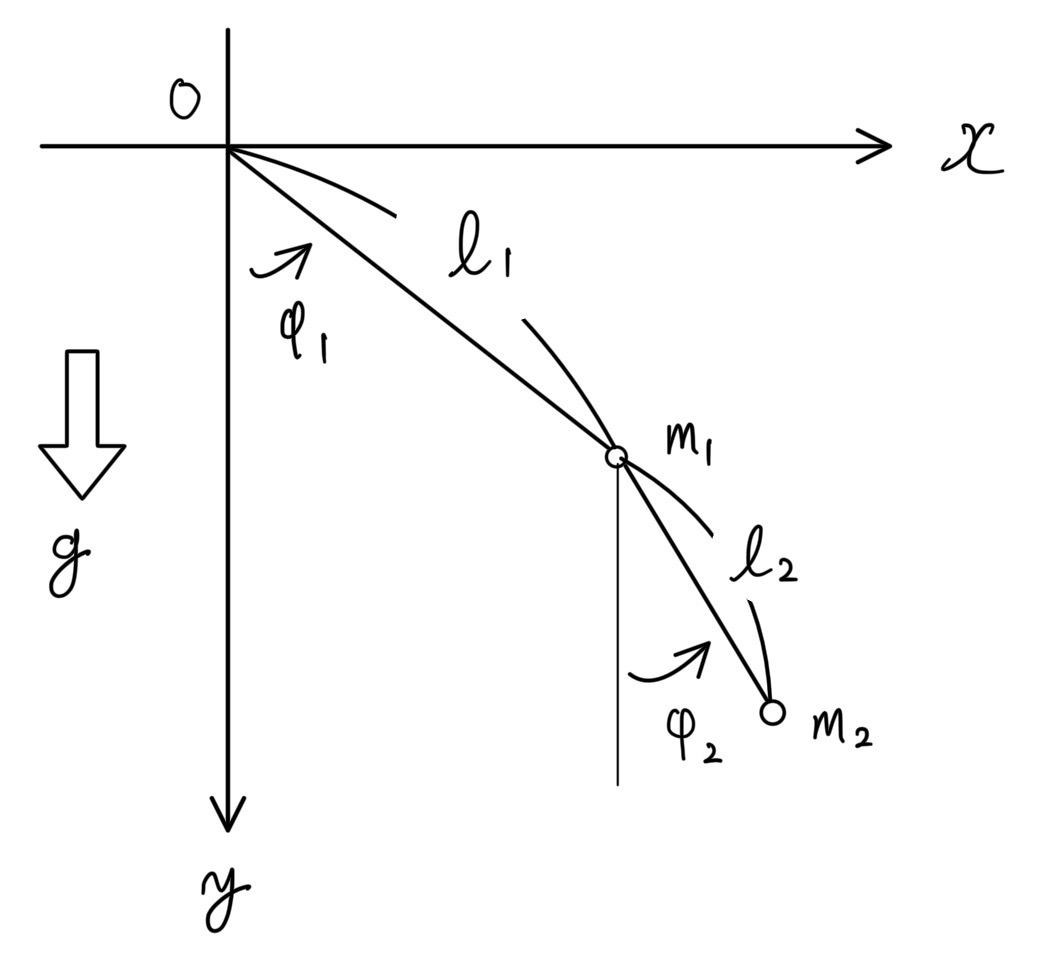
\includegraphics[width=0.9\textwidth]{1.png}
        \caption{2重振り子}
        \label{fig:1}
    \end{minipage}
    \begin{minipage}[b]{0.49\textwidth}
        \centering
        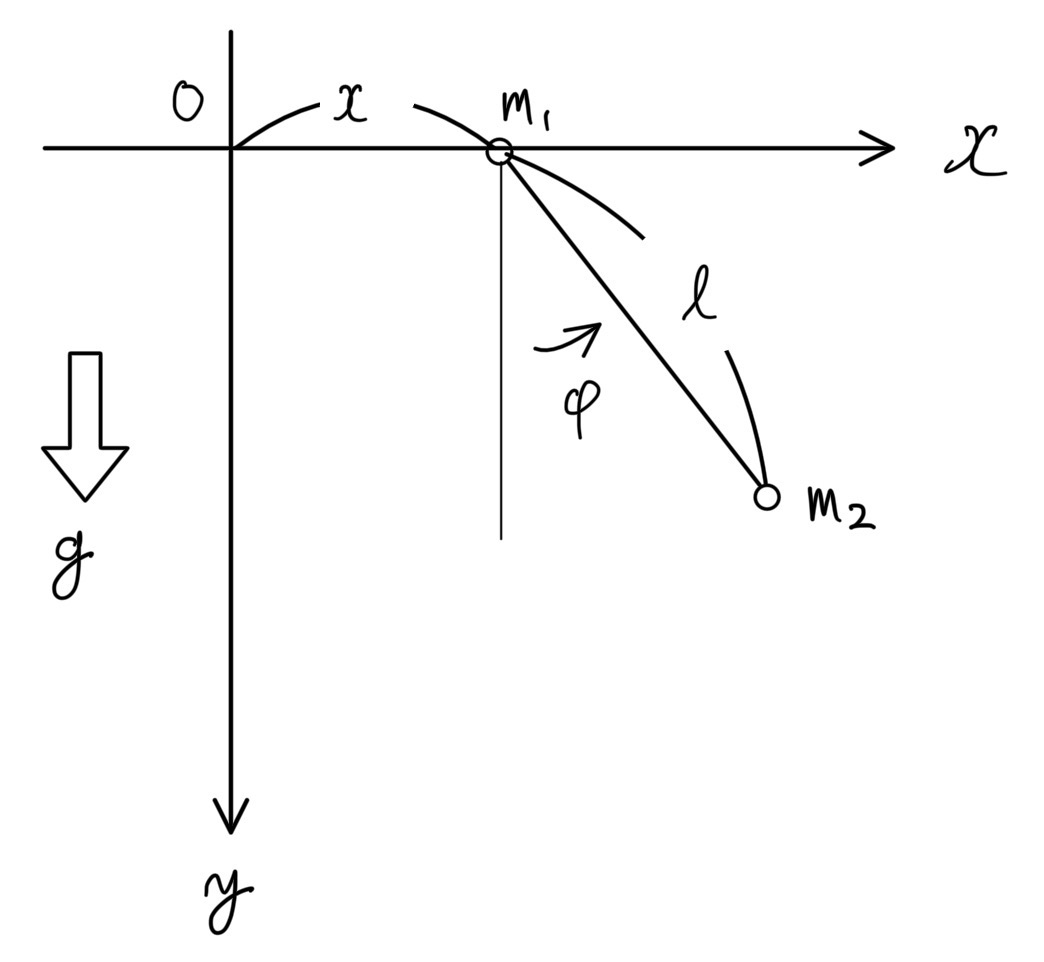
\includegraphics[width=0.9\textwidth]{2.png}
        \caption{支点が動く1重振り子}
        \label{fig:2}
    \end{minipage}
  \end{figure}

  \part{中心力場中の1粒子の問題}

  \section{Q2A-3（中心力場中の1粒子の運動）}
  3次元空間内の質量mの質点が、原点Oを対称性の中心とする中心力ポテンシャル$V(\vect{r})=V(|\vect{r}|)$のもとで運動するとする。
  \subsection*{(i)}
  質点の座標を球座標で表したときのLagrange関数を求める。\\
  第一に、ポテンシャルエネルギーは中心力ポテンシャルであるので、$V(\vect{r})=V(r)$と書ける。次に運動エネルギー$T$を、線素を用いて求める：
  \begin{align*}
    T=\frac{m}{2}\left|\bbn{\vect{r}}{t}\right|^2=\frac{m}{2}\left|\frac{d\vect{l}}{dt}\right|^2=\frac{m}{2}\left|\frac{1}{dt}\vectxyz{dr}{rd\theta}{r\sin\theta d\varphi}\right|^2=\frac{m}{2}\left|\vectxyz{\dot{r}}{r\dot{\theta}}{r\sin\theta\dot{\varphi}}\right|^2=\frac{1}{2}m\left(\dot{r}^2+r^2\dot{\theta}^2+r^2\sin^2\theta\dot{\varphi}^2\right)。
  \end{align*}
  したがって、この質点のLagrange関数Lは次のようになる：
  \begin{align*}
    L=T-V(r)=\frac{1}{2}m\left(\dot{r}^2+r^2\dot{\theta}^2+r^2\sin^2\theta\dot{\varphi}^2\right)-V(r)。\tag{11}
  \end{align*}
  \subsection*{(ii)}
  $\theta$の運動の追跡をする。\\
  初期時刻$t=0$での粒子の位置ベクトル$\vect{r}$と速度ベクトル$\vect{\dot{\vect{r}}}$の両者が球座標の赤道の平面$\theta=\frac{\pi}{2}$に含まれるように、球座標の極軸$\theta=0$の方向を$+\vect{r}\times\dot{\vect{r}}$に定める。
  この初期条件をまとめると、
  \begin{align*}
    \left\{
    \begin{aligned}
      \theta(0)&=\frac{\pi}{2}\\
      \dot{\theta}(0)&=0
    \end{aligned}
    \right.
  \end{align*}
  である。\\
  上で求めたLagrange関数Lを一般座標$\theta$についてのEuler-Lagrange方程式に代入する：
  \begin{align*}
    \bbn{}{t}\left(\hb{L}{\dot{\theta}}\right)&=\hb{L}{\theta}\\
    \therefore m\left(2r\dot{r}\dot{\theta}+r^2\ddot{\theta}\right)&=2r^2\sin\theta\cos\theta\dot{\varphi}^2。
  \end{align*}
  $\theta(t)=\frac{\pi}{2}$はこの微分方程式を満たすため、解の一つであることがわかる。さらに、これは初期条件与えられた初期条件も満たすためただ一つの解である。\\
  以上より、$\theta=\frac{\pi}{2}$の一定値にとどまることが示された：\\
  \begin{align*}
    \theta=\frac{\pi}{2}\quad(t\geq0)\tag{12}
  \end{align*}
  任意の初期値$\vect{r}(0),\dot{\vect{r}}(0)$に対して同様に$\vect{r}(0)\times\dot{\vect{r}}(0)$に平行に極軸を取れば、同じことが成り立つ。つまり、質点の運動は$\mathrm{Span}\{\vect{r}(0),\dot{\vect{r}}(0)\}$上に限られるというわけだ。
  \subsection*{(iii)}
  2次元極座標でのLagrange関数を求める。ポテンシャルエネルギーは球座標と同様であり、変化する部分は運動エネルギーTである。これは線素を用いれば直ちに求まる：
  \begin{align*}
    T=\frac{m}{2}\left|\bbn{\vect{r}}{t}\right|^2=\frac{m}{2}\left|\frac{d\vect{l}}{dt}\right|^2=\frac{m}{2}\left|\frac{1}{dt}\vectxy{dr}{rd\varphi}\right|^2=\frac{m}{2}\left|\vectxy{\dot{r}}{r\dot{\varphi}}\right|^2=\frac{1}{2}m\left(\dot{r}^2+r^2\dot{\varphi}^2\right)。
  \end{align*}
  よって、Lagrange関数Lは次のようになる：
  \begin{align*}
    L=T-V(r)=\frac{1}{2}m\left(\dot{r}^2+r^2\dot{\varphi}^2\right)-V(r)。\tag{13}
  \end{align*}
  \subsection*{(iv)}
  保存量について考える。上で求めたLagrange関数LをEuler-Lagrange方程式に代入する：
  \begin{alignat*}{2}
    &\phantom{=}  &\bbn{}{t}\left(\hb{L}{\dot{\varphi}}\right)&=\hb{L}{\varphi}\\
    &\phantom{=}  \therefore \,&\bbn{}{t}\left(mr^2\dot{\varphi}\right)&=0\\
    &\phantom{=}  \therefore \,&mr^2\dot{\varphi}&=(一定)\quad(t\geq0)。\tag{14}
  \end{alignat*}
  この左辺を一般座標$\varphi$に対応した一般運動量$p_\varphi$と呼ぶのである。以上より、$p_\varphi$が時間的に保存されることが示された。
  \subsection*{(v)}
  Descartes座標での運動量$\vect{p}$は、$r,\varphi$を用いて表すと次のようになる：
  \begin{align*}
    \vect{p} =m\bbn{r}{t}=m\bbn{}{t}\vectxyz{r\cos\varphi}{r\sin\varphi}{0}=\vectxyz{m\dot{r}\cos\varphi-mr\dot{\varphi}\sin\varphi}{m\dot{r}\sin\varphi+mr\dot{\varphi}\cos\varphi}{0}。
  \end{align*}
  よって、角運動量$\vect{l}$は位置ベクトルを左から外積すれば求められる：
  \begin{align*}
    \boldsymbol{l}=\vect{r}\times\vect{p}&=\vectxyz{r\cos\varphi}{r\sin\varphi}{0}\times\vectxyz{m\dot{r}\cos\varphi-mr\dot{\varphi}\sin\varphi}{m\dot{r}\sin\varphi+mr\dot{\varphi}\cos\varphi}{0}\\
    &=\vectxyz{0}{0}{mr^2\dot{\varphi}}\\
    \therefore l_z &= mr^2\dot{\varphi}=p_\varphi。\tag{15}
  \end{align*}
  したがって、一般運動量$p_\varphi$は、角運動量のz軸方向成分$l_z$に他ならないことが示された。

  \subsection*{(vi)}
  角運動量ベクトルと一般運動量の大きさが等しいことを示す：
  \begin{align*}
    l^2=|\boldsymbol{l}|^2=\left|\vectxyz{0}{0}{mr^2\dot{\varphi}}\right|^2=\left(mr^2\dot{\varphi}\right)^2=p_\varphi^2。\tag{16}
  \end{align*}
  以上より両者が等しいことが示された。

  \subsection*{(vii)}
  循環座標$\varphi$を消去することで修正されたLagrange関数$\hat{L}$を求める。まず(13)式の$L$を次のように書き換える：
  \begin{align*}
    L=\frac{1}{2}m\left(\dot{r}^2+r^2\dot{\varphi}^2\right)-V(r)=\frac{1}{2}m\dot{r}^2+\frac{m^2r^4\dot{\varphi}^2}{2mr^2}-V(r)=\frac{1}{2}m\dot{r}^2+\frac{l^2}{2mr^2}-V(r)。
  \end{align*}
  これを修正するために、$\varphi$が循環座標であることを用いる。(14)式より$p_\varphi$は時間的に保存される。よって$\frac{l^2}{mr^2}=mr^2\dot{\varphi}^2=p_\varphi \dot{\varphi}=\bbn{}{t}(p_\varphi \varphi)$は、関数$p_\varphi \varphi$の時間についての完全導関数であるため、Lagrange関数に加えてもよい。よってこれを引いたものを新たにLagrange関数$\hat{L}$とおく：
  \begin{align*}
    \hat{L}=L-p_\varphi \varphi=\frac{1}{2}m\dot{r}^2+\frac{l^2}{2mr^2}-V(r)-\frac{l^2}{mr^2}=\frac{1}{2}m\dot{r}^2-\frac{l^2}{2mr^2}-V(r)=\frac{1}{2}m\dot{r}^2-V_{\mathrm{eff}}(r)。\tag{17}
  \end{align*}
  ここで、有効ポテンシャル$V_{\mathrm{eff}}(r)$は次のように定める：
  \begin{align*}
    V_{\mathrm{eff}}(r)=V(r)+\frac{l^2}{2mr^2}。\tag{18}
  \end{align*}

  \subsection*{(viii)}
  保存法則の導出をする。\\
  時間の一様性から、孤立系のLagrange関数$\hat{L}$は時間に陽に依存することはない。したがって、Lagrange関数の時間に関する完全導関数はChain Ruleを用いて次の形に書ける：
  \begin{align*}
    \bbn{\hat{L}}{t}=\hb{\hat{L}}{\dot{r}}\ddot{r}+\hb{\hat{L}}{r}\dot{r}。
  \end{align*}
  導関数$\hb{\hat{L}}{r}$をEuler-Lagrange方程式に従って$\bbn{}{t}\hb{\hat{L}}{\dot{r}}$と書き直せば、
  \begin{align*}
    &\phantom{=}\bbn{\hat{L}}{t}=\hb{\hat{L}}{\dot{r}}\ddot{r}+\dot{r}\bbn{}{t}\hb{\hat{L}}{\dot{r}}=\bbn{}{t}\left(\hb{\hat{L}}{\dot{r}}\dot{r}\right)\\
    &\phantom{=}\therefore \bbn{}{t}\left(\hb{\hat{L}}{\dot{r}}\dot{r}-\hat{L}\right)=0\\
    &\phantom{=}\therefore \bbn{}{t}\left(\frac{1}{2}m\dot{r}^2+\frac{l^2}{2mr^2}+V(r)\right)=0\\
    &\phantom{=}\therefore \frac{1}{2}m\dot{r}^2+\frac{l^2}{2mr^2}+V(r)=(一定)。
  \end{align*}
  以上より不変量として、次の運動の積分Eが得られた：
  \begin{align*}
    E=\frac{1}{2}m\dot{r}^2+\frac{l^2}{2mr^2}+V(r)。\tag{19}
  \end{align*}

  \subsection*{(ix)}
  (viii)で得られた運動の積分$E$が、3次元空間を運動する粒子の全エネルギーに等しいことを確認する。\\
  中心力場中の粒子の運動は平面内に限られるので、その平面上の極座標$(r,\phi)$を用いて運動エネルギーを書くことができる。このとき、3次元空間での全エネルギー$E_{\mathbb{R}^3}$は運動エネルギーとポテンシャルエネルギーの和として次のように表される：
  \begin{align*}
    E_{\mathbb{R}^3}
    &= T + V(r)\\
    &= \frac12 m\left(\dot r^2+r^2\dot\varphi^2\right)+V(r) \\
    &= \frac12 m\dot r^2+\frac12 mr^2\dot\varphi^2+V(r)\\
    &=\frac12m\dot r^2 +\frac{l^2}{2mr^2}+V(r)。
  \end{align*}
  これは(viii)で得られた運動の積分$E$と一致する。以上より、(19)式に現れた定数$E$は、3次元空間を運動する粒子の全エネルギーであることが示された。

  \subsection*{(x)}
  (19)式を積分し、動径座標$r$と時間$t$の関係を導く。\\
  まず(19)式を$\dot{r}$について解く：
  \begin{align*}
    &\phantom{=} E=\frac{1}{2}m\dot{r}^2+\frac{l^2}{2mr^2}+V(r)\\
    &\phantom{=}\therefore \dot r^2=\frac2m\left(E-V(r)\right)-\frac{l^2}{m^2r^2}\\
    &\phantom{=}\therefore \dot r=\sqrt{\frac2m\left(E-V(r)\right)-\frac{l^2}{m^2r^2}}。
  \end{align*}
  また、$\dot r=\bbn{r}{t}\therefore dt=\frac{dr}{\dot{r}}$であるから、
  \begin{align*}
    dt=\frac{dr}{\dot{r}}=\frac{dr}{\sqrt{\frac2m\left(E-V(r)\right)-\frac{l^2}{m^2r^2}}}。\tag{20.0}
  \end{align*}
  この両辺を積分する:
  \begin{align*}
    &\phantom{=}\int dt = \int\frac{dr}{\sqrt{\frac2m\left(E-V(r)\right)-\frac{l^2}{m^2r^2}}}\\
    &\phantom{=}\therefore t = \int \frac{dr}{\sqrt{\frac2m\left(E-V(r)\right)-\frac{l^2}{m^2r^2}}} + (定数)。\tag{20}
  \end{align*}
  以上より動径座標$r$と時間$t$の関係が導かれた。
  
  \subsection*{(xi)}
  次に、$t$から$\varphi$への変数変換を考える。まずは、$dt$と$d\varphi$の関係$d\varphi=\frac{l}{mr^2}dt$を導く。$\dot{\varphi}\geq0$であるとすれば、15式から次のようになる：
  \begin{align*}
    mr^2\dot{\varphi}=l \therefore d\varphi=\frac{l}{mr^2}dt。\tag{21}
  \end{align*}

  \subsection*{(xii)}
  (20.0)式を(21)式に代入する：
  \begin{align*}
    d\varphi=\frac{l}{mr^2}dt=\frac{l}{mr^2}\frac{dr}{\sqrt{\frac2m\left(E-V(r)\right)-\frac{l^2}{m^2r^2}}}=\frac{\frac{l}{r^2}dr}{\sqrt{2m\left(E-V(r)\right)-\frac{l^2}{r^2}}}。
  \end{align*}
  この両辺を積分する:
  \begin{align*}
    \int d\varphi = \int \frac{\frac{l}{r^2}dr}{\sqrt{2m\left(E-V(r)\right)-\frac{l^2}{r^2}}}\\
    \therefore \varphi = \int \frac{\frac{l}{r^2}dr}{\sqrt{2m\left(E-V(r)\right)-\frac{l^2}{r^2}}} + (定数)。\tag{22}
  \end{align*}
  以上より動径座標と$r$と角度座標$\varphi$の関係が導かれた。

  \section{Q2A-4（Keplerの第二法則）}
  (21)式から、Keplerの第二法則を示す。\\
  まず、面積速度$\dot{S}$とは次のような量をいう：
  \begin{align*}
    \dot{S}=\frac{1}{2}\left|\vect{r}\times\dot{\vect{r}}\right|。
  \end{align*}
  2次元極座標では速度ベクトルは$\dot{\vect{r}}=\vectxy{\dot{r}}{r\dot{\varphi}}$であるから、面積速度は次のようになる：
  \begin{align*}
    \dot{S}=\frac{1}{2}\left|\vect{r}\times\dot{\vect{r}}\right|=\frac{1}{2}\left|\vectxyz{r\cos\varphi}{r\sin\varphi}{0}\times\vectxyz{\dot{r}\cos\varphi-r\dot{\varphi}\sin\varphi}{r\dot{r}\sin\varphi+r\dot{\varphi}\cos\varphi}{0}\right|=\frac{1}{2}r^2\dot{\varphi}。
  \end{align*}
  ここに(21)式を代入する：
  \begin{align*}
    \dot{S}=\frac{1}{2}r^2\dot{\varphi}=\frac{1}{2}r^2\frac{l}{mr^2}=\frac{l}{2m}。
  \end{align*}
  これは定数である。したがって、面積速度は一定である。以上より、Keplerの第二法則が示された。

  \part{Kepler問題：基本}

  \section{Q2A-5（Kepler問題：引力の場合、負のエネルギー$E<0$）}
  次の中心力ポテンシャル$V(r)$を受けて3次元空間を運動する質量mの1粒子を考える：
  \begin{align*}
    V(r)=-\frac\alpha r。\tag{23}
  \end{align*}
  ただし、$\alpha$は正の定数である：$\alpha>0$。この問題では、\hyperref[fig:3]{図3}を参考にしてください。

  \subsection*{(i)}
  有効ポテンシャル
  \begin{align*}
    V_{\mathrm{eff}}(r)=V(r)+\frac{l^2}{2mr^2}=-\frac\alpha r +\frac{l^2}{2mr^2}\tag{24}
  \end{align*}
  について、次の事実を確かめる：\\
  ・$r\downarrow +0$のとき、$V_{\mathrm{eff}}(r)$は$+\infty$に発散する：
  \begin{align*}
    \lim_{r\downarrow +0}V_{\mathrm{eff}}(r)=+\infty。\tag{25}
  \end{align*}
  ・$r\uparrow+\infty$のとき、$V_{\mathrm{eff}}(r)$は0へ下から漸近する：
  \begin{align*}
    \lim_{r\uparrow +\infty}V_{\mathrm{eff}}(r)=0(下から)。\tag{26}
  \end{align*}
  ・$r=\frac{l^2}{\alpha m}$において、$V_{\mathrm{eff}}(r)$は最小値$-\frac{\alpha^2 m}{2l^2}$を取る：
  \begin{align*}
    -\frac{\alpha^2 m}{2l^2}=V_{\mathrm{eff}}(\frac{l^2}{\alpha m})\leq V_{\mathrm{eff}}(r)\quad(0<r<+\infty)。\tag{27}
  \end{align*}
  まず$r\downarrow +0$の極限を考える。全体を$r^2$でくくる：
  \begin{align*}
    \lim_{r\downarrow+0}V_{\mathrm{eff}}(r)=\lim_{r\downarrow+0}\frac{1}{r^2}\left(-r\alpha + \frac{l^2}{2m}\right)=\lim_{r\downarrow+0}\frac{1}{r^2}\left(\frac{l^2}{2m}\right)=+\infty
  \end{align*}
  よって(25)式は正しい。\\
  次に、$r\uparrow+\infty$の極限を考える。$V_{\mathrm{eff}}(r)<0$を解くと$\frac{l^2}{2m\alpha}<r$である。よってこの極限では$V_{\mathrm{eff}}(r)<0$として良い。
  \begin{align*}
    \lim_{r\uparrow+\infty}V_{\mathrm{eff}}(r)=0+0=0
  \end{align*}
  であり、また十分大きな$r$に対して$V_{\mathrm{eff}}(r)<0$であるため、$V_{\mathrm{eff}}(r)$は0に下から漸近する。よって(26)式も確認できた。\\
  最後に、最小値を考える。$V_{\mathrm{eff}}(r)$を$r$で微分すると、$\dot{V_{\mathrm{eff}}(r)}=\frac{\alpha}{r^2}-\frac{l^2}{mr^3}$である。
  \begin{align*}
    \dot{V_{\mathrm{eff}}(r)}=\frac{\alpha}{r^2}-\frac{l^2}{mr^3}\gtreqqless 0\iff r \gtreqqless \frac{l^2}{\alpha m}
  \end{align*}
  であるため、$r=\frac{l^2}{\alpha m}$において、$V_{\mathrm{eff}}(r)$は最小値$-\frac{\alpha^2 m}{2l^2}$を取る。(27)式も確認できた。

  \subsection*{(ii)}
  (i)における議論を踏まえて、$V_{\mathrm{eff}}(r)$のグラフの概形を書くと下図のようになる。

  \begin{figure}[h]
    \centering
    \begin{tikzpicture}[x=1.2cm,y=3.2cm]
      % 軸
      \draw[->] (0,0) -- (6.2,0) node[right] {$r$};
      \draw[->] (0,-0.45) -- (0,1.35) node[above] {$V_{\mathrm{eff}}(r)$};
      % グラフ本体だけを表示範囲内に収める
      \begin{scope}
        \clip (0,-0.45) rectangle (6.2,1.35);
        \draw[thick, domain=0.45:6.0, samples=300, smooth]
          plot (\x, {-1/(\x) + 1/(\x*\x)});
      \end{scope}
      % 最小点
      \fill (2,-0.25) circle (1.2pt);
    \end{tikzpicture}
    \caption*{有効ポテンシャル$V_{\mathrm{eff}}$のグラフ}
    \label{fig:veff}
  \end{figure}

  \subsection*{(iii)}
  全エネルギー$E$が正またはゼロならば、最終的に粒子は無限遠$r=\infty$に飛び去ってしまい、運動が有界ではないことを示す。\\
  全エネルギー$E$は運動エネルギー$T=\frac12 m\dot{r}^2$と有効ポテンシャル$V_{\mathrm{eff}}(r)$の和として$E=T+V_{\mathrm{eff}}(r)$と表される。粒子の存在条件は$T\geq0$であるから、$T=E-V_{\mathrm{eff}}(r)\geq0\therefore E\geq V_{\mathrm{eff}}(r)$である。\\
  上で示したように、有効ポテンシャルは$r\uparrow +\infty$において$0$に下から漸近する。よって、$E\geq0$であれば、十分大きな$r$に対して$0>V_{\mathrm{eff}}(r)$であるため、$E\geq V_{\mathrm{eff}}(r)$を満たす。したがって、粒子は$r=\infty$に到達できる。\\
  以上のことから次の事が示された：
  \begin{align*}
    E\geq0\iff 「粒子の運動は有界でない。」。\tag{28}
  \end{align*}

  \subsection*{(iv)}
  全エネルギー$E$が負であるならば、粒子の運動は有界であり、動径座標$r$は時間$t$に関して周期的になることを示す。
  グラフからもわかる通り、$\min\{V_{\mathrm{eff}}(r)\}\leq E < 0\Longleftrightarrow -\frac{\alpha^2 m}{2l^2}\leq E < 0$であれば、$E=V_{\mathrm{eff}}(r)$は2つの実数根をもつ。これらをそれぞれ$r_{\min},r_{\max}\,(r_{\min}\leq r_{\max})$とおくと、粒子の存在条件は以下のようになる：
  \begin{align*}
    E\geq \veff\Longleftrightarrow r_{\min}\leq r \leq r_{\max}。
  \end{align*}
  また、動径方向の運動は1次元の有効ポテンシャル中の運動として見られるので、粒子は$r_{\min}$と$r_{\max}$の間を往復する。したがって、動径座標$r$は時間$t$に関して周期的になる。以上より、以下のことが示された：
  \begin{align*}
    -\frac{\alpha^2 m}{2l^2}\leq E < 0 \iff 「粒子の運動は有界であり、動径座標rは時間tに関して周期的である。」。\tag{29}
  \end{align*}
  この問題では以降、エネルギー$E$が負である場合、
  \begin{align*}
    -\frac{\alpha^2 m}{2l^2}\leq E<0\tag{30}
  \end{align*}
  を考えることとする。
  
  \subsection*{(v)}
  ここでは、(22)式に具体的なポテンシャルを代入し、軌跡の方程式を計算する。\\
  (22)式に$V(r)=-\frac{\alpha}{r}$を代入する：
  \begin{align*}
    \varphi=\int \frac{\frac{l}{r^2}\,dr}{\sqrt{2m\left(E+\frac{\alpha}{r}\right)-\frac{l^2}{r^2}}}+(定数)。
  \end{align*}
  ここで$u=1/r$とおくと、$du=-dr/r^2$であるから、積分は次のように書き換えられる：
  \begin{align*}
    \varphi=-\int\frac{l\,du}{\sqrt{2mE+2m\alpha u-l^2u^2}}+(定数)。
  \end{align*}
  根号内を平方完成する：
  \begin{align*}
    2mE+2m\alpha u-l^2u^2=2mE+\frac{m^2\alpha^2}{l^2}-\left(lu-\frac{m\alpha}{l}\right)^2。
  \end{align*}
  したがって、積分は次のようになる：
  \begin{align*}
    \varphi=-\int\frac{l\,du}{\sqrt{2mE+\frac{m^2\alpha^2}{l^2}-\left(lu-\frac{m\alpha}{l}\right)^2}}+(定数)。
  \end{align*}
  ここで、
  \begin{align*}
    w=\frac{lu-\frac{m\alpha}{l}}{\sqrt{2mE+\frac{m^2\alpha^2}{l^2}}}
  \end{align*}
  とおくと、
  \begin{align*}
    dw=\frac{l\,du}{\sqrt{2mE+\frac{m^2\alpha^2}{l^2}}}
  \end{align*}
  である。よって、積分は次のように実行できる：
  \begin{align*}
    \varphi=-\int\frac{dw}{\sqrt{1-w^2}}+(定数)=\arccos w+(定数)。
  \end{align*}
  最後に$w$を代入したうえで$u=\frac1r$を戻すことで、軌跡の方程式は次のように得られる：
  \begin{align*}
    \varphi=\arccos\frac{\frac{l}{r}-\frac{m\alpha}{l}}{\sqrt{2mE+\frac{m^2\alpha^2}{l^2}}}+(定数)。\tag{31}
  \end{align*}

  \subsection*{(vi)}
  (31)式が次のように整理されることを示す：
  \begin{align*}
    r=\frac{p}{1+e\cos\varphi}。\tag{32}
  \end{align*}
  積分定数が0となるように、$\varphi=0$の方向を選ぶ。このとき、(31)式は次を意味する：
  \begin{align*}
    \cos\varphi=\frac{\frac{l}{r}-\frac{m\alpha}{l}}{\sqrt{2mE+\frac{m^2\alpha^2}{l^2}}}。
  \end{align*}
  これを$r$について整理する：
  \begin{align*}
    \frac{1}{r}=\frac{m\alpha}{l^2}+\frac{1}{l}\sqrt{2mE+\frac{m^2\alpha^2}{l^2}}\cos\varphi。
  \end{align*}
  ここで、パラメータ$p,e$を次のように定める：
  \begin{align*}
    p&=\frac{l^2}{m\alpha},\tag{33}\\
    e&=\frac{l}{m\alpha}\sqrt{2mE+\frac{m^2\alpha^2}{l^2}}=\sqrt{1+\frac{2El^2}{m\alpha^2}}。\tag{34}
  \end{align*}
  この定義を用いると、上式は次のように書ける：
  \begin{align*}
    \frac{1}{r}=\frac{1}{p}(1+e\cos\varphi)。
  \end{align*}
  したがって、(31)式は次のように整理される：
  \begin{align*}
    r=\frac{p}{1+e\cos\varphi}。
  \end{align*}
  以上より、(32)式が示された。

  \subsection*{(vii)}
  ここでは、(32)式が原点を焦点とする楕円を表すことを、楕円の標準形に変形することにより示す。その後、通径、離心率、近日点の定義に基づいて、$p,e,\varphi=0$の意味を確認する。まず、今は負のエネルギー$E<0$の場合を考えているので、(34)式より次が成り立つ：
  \begin{align*}
    e^2=1+\frac{2El^2}{m\alpha^2}<1。
  \end{align*}
  また、エネルギー$E$は有効ポテンシャルの最小値以上であるから、$e^2\geq0$である。したがって、
  \begin{align*}
    0\leq e<1
  \end{align*}
  である。ここで、極座標とDescartes座標の関係$x=r\cos\varphi,\ y=r\sin\varphi$を用いる。(32)式の両辺に$1+e\cos\varphi$を掛ける：
  \begin{align*}
    r+ex=p。
  \end{align*}
  さらに$r^2=x^2+y^2$であるから、両辺を2乗して整理する：
  \begin{align*}
    x^2+y^2=(p-ex)^2=p^2-2pex+e^2x^2,\qquad \therefore (1-e^2)x^2+y^2+2pex-p^2=0。
  \end{align*}
  これを$x$について平方完成する：
  \begin{align*}
    (1-e^2)\left(x+\frac{pe}{1-e^2}\right)^2+y^2=\frac{p^2}{1-e^2}。
  \end{align*}
  両辺を右辺で割ると、次の標準形を得る：
  \begin{align*}
    \frac{\left(x+\frac{pe}{1-e^2}\right)^2}{\left(\frac{p}{1-e^2}\right)^2}+\frac{y^2}{\frac{p^2}{1-e^2}}=1。
  \end{align*}
  ここで、
  \begin{align*}
    a=\frac{p}{1-e^2},\qquad b=\frac{p}{\sqrt{1-e^2}}
  \end{align*}
  とおけば、
  \begin{align*}
    \frac{\left(x+\frac{pe}{1-e^2}\right)^2}{a^2}+\frac{y^2}{b^2}=1
  \end{align*}
  である。これは中心が$\left(-\frac{pe}{1-e^2},0\right)$にあり、長半径$a$、短半径$b$をもつ楕円の標準形である。したがって、(32)式は楕円を表すことが示された。

  次に、この楕円の焦点を調べる。楕円の焦点距離$c$は$c^2=a^2-b^2$で定義されるので、上で得た$a,b$を代入する：
  \begin{align*}
    c^2=\left(\frac{p}{1-e^2}\right)^2-\frac{p^2}{1-e^2}=\frac{p^2e^2}{(1-e^2)^2},\therefore c=\frac{pe}{1-e^2}。
  \end{align*}
  楕円の中心は$\left(-\frac{pe}{1-e^2},0\right)=(-c,0)$であり、長軸は$x$軸方向である。したがって、2つの焦点は
  \begin{align*}
    (-c+c,0)=(0,0),\qquad (-c-c,0)=(-2c,0)
  \end{align*}
  である。よって、原点はこの楕円の焦点の一つである。以上より、(32)式は原点を焦点とする楕円の方程式であることが示された。

  離心率は、楕円の中心から焦点までの距離$c$を長半径$a$で割った量として定義される。したがって、この楕円の離心率は次のようになる：
  \begin{align*}
    \frac{c}{a}=\frac{\frac{pe}{1-e^2}}{\frac{p}{1-e^2}}=e。
  \end{align*}
  よって、(32)式に現れる$e$は楕円の離心率である。

  次に、通径について確認する。ここでは、焦点を通り長軸に垂直な直線が楕円と交わる点までの焦点からの距離を通径と呼ぶことにする。原点を焦点として見たとき、長軸は$x$軸方向であるから、通径の方向は$\varphi=\frac{\pi}{2}$または$\varphi=\frac{3\pi}{2}$である。したがって、(32)式に$\cos\varphi=0$を代入する：
  \begin{align*}
    r=\frac{p}{1+e\cdot0}=p。
  \end{align*}
  よって、$p$は焦点から通径の端点までの距離を表している。この意味で、(32)式に現れる$p$は楕円の通径である。

  最後に、近日点の方向を確認する。近日点とは、力の中心である焦点からの距離$r$が最小となる軌道上の点である。$0\leq e<1$であるから、$r$が最小となるのは(32)式において分母が最大となるときである。分母は$\cos\varphi=1$のとき最大となるので、
  \begin{align*}
    \varphi=0
  \end{align*}
  の方向が近日点の方向である。以上より、$p$は通径、$e$は離心率、$\varphi=0$は焦点から見た近日点の方向であることが示された。

  \subsection*{(viii)}
  ここでは、軌道の長半径$a$と短半径$b$を求める。前小問で得た楕円の標準形から、長半径と短半径は次のように読める：
  \begin{align*}
    a=\frac{p}{1-e^2},\qquad b=\frac{p}{\sqrt{1-e^2}}。
  \end{align*}
  ここに$p=\frac{l^2}{m\alpha}$と$e^2=1+\frac{2El^2}{m\alpha^2}$を代入する。今は$E<0$であるから、$\left|E\right|=-E$であり、
  \begin{align*}
    1-e^2=-\frac{2El^2}{m\alpha^2}=\frac{2\left|E\right|l^2}{m\alpha^2}
  \end{align*}
  である。したがって、長半径$a$は次のように求まる：
  \begin{align*}
    a=\frac{\frac{l^2}{m\alpha}}{\frac{2\left|E\right|l^2}{m\alpha^2}}=\frac{\alpha}{2\left|E\right|}。
  \end{align*}
  同様に、短半径$b$は次のように求まる：
  \begin{align*}
    b=\frac{\frac{l^2}{m\alpha}}{\sqrt{\frac{2\left|E\right|l^2}{m\alpha^2}}}=\frac{l}{\sqrt{2m\left|E\right|}}。
  \end{align*}
  以上より、
  \begin{align*}
    a&=\frac{p}{1-e^2}=\frac{\alpha}{2\left|E\right|},\tag{35}\\
    b&=\frac{p}{\sqrt{1-e^2}}=\frac{l}{\sqrt{2m\left|E\right|}}。\tag{36}
  \end{align*}
  特に、長半径$a$はエネルギー$E$のみで決まり、角運動量の大きさ$l$には依存しない。

  \subsection*{(ix)}
  ここでは、全エネルギー$E$が可能な最小値を取るとき、軌跡が円になることを示す。エネルギーが可能な最小値
  \begin{align*}
    E=-\frac{\alpha^2m}{2l^2}
  \end{align*}
  を取るとき、離心率$e$は次のようになる：
  \begin{align*}
    e=\sqrt{1+\frac{2\left(-\frac{\alpha^2m}{2l^2}\right)l^2}{m\alpha^2}}=0。
  \end{align*}
  このとき、軌跡の方程式(32)式は
  \begin{align*}
    r=p
  \end{align*}
  となる。これは原点を中心とする円を表す。したがって、エネルギーが可能な最小値を取るとき、離心率は$0$となり、軌跡の楕円は円になることが示された。

  \subsection*{(x)}
  ここでは、動径座標$r$の最小値$r_{\min}$と最大値$r_{\max}$を求める。$0\leq e<1$であるから、$r$が最小となるのは(32)式において分母が最大となるとき、すなわち$\cos\varphi=1$のときである。したがって、
  \begin{align*}
    r_{\min}=\frac{p}{1+e}
  \end{align*}
  である。一方、$r$が最大となるのは分母が最小となるとき、すなわち$\cos\varphi=-1$のときである。したがって、
  \begin{align*}
    r_{\max}=\frac{p}{1-e}
  \end{align*}
  である。ここで$a=\frac{p}{1-e^2}$を用いると：
  \begin{align*}
    a(1-e)=\frac{p}{1+e},\qquad a(1+e)=\frac{p}{1-e}。
  \end{align*}
  よって、動径座標の最小値と最大値は次である：
  \begin{align*}
    r_{\min}&=\frac{p}{1+e}=a(1-e),\tag{37}\\
    r_{\max}&=\frac{p}{1-e}=a(1+e)。\tag{38}
  \end{align*}

  \subsection*{(xi)}
  ここでは、楕円軌道を一周する周期$T$を求める。Q2A-4で示したKeplerの第2法則より、面積速度は一定である：
  \begin{align*}
    \dot{S}=\frac{l}{2m}。
  \end{align*}
  また、長半径$a$、短半径$b$の楕円の面積は$\pi ab$である。したがって、一周期$T$は次で与えられる：
  \begin{align*}
    T=\frac{\pi ab}{\frac{l}{2m}}=\frac{2\pi mab}{l}。
  \end{align*}
  ここに$b=\frac{l}{\sqrt{2m\left|E\right|}}$を代入する：
  \begin{align*}
    T=\frac{2\pi ma}{l}\frac{l}{\sqrt{2m\left|E\right|}}=2\pi a\sqrt{\frac{m}{2\left|E\right|}}。
  \end{align*}
  さらに、(35)式より$a=\frac{\alpha}{2\left|E\right|}$であるから、$\left|E\right|=\frac{\alpha}{2a}$である。これを代入する：
  \begin{align*}
    T=2\pi a\sqrt{\frac{m}{2\cdot\frac{\alpha}{2a}}}=2\pi a^{3/2}\sqrt{\frac{m}{\alpha}}。
  \end{align*}
  また、$a=\frac{\alpha}{2\left|E\right|}$を用いて$T$をエネルギーで表す：
  \begin{align*}
    T=2\pi\frac{\alpha}{2\left|E\right|}\sqrt{\frac{m}{2\left|E\right|}}=\pi\alpha\sqrt{\frac{m}{2\left|E\right|^3}}。
  \end{align*}
  以上より、周期$T$は次のように計算された：
  \begin{align*}
    T=2\pi a^{3/2}\sqrt{\frac{m}{\alpha}}=\pi\alpha\sqrt{\frac{m}{2\left|E\right|^3}}。\tag{39}
  \end{align*}

  \subsection*{(xii)}
  最後に、(39)式からKeplerの第3法則を導く。(39)式より、周期$T$は次のように表される：
  \begin{align*}
    T=2\pi a^{3/2}\sqrt{\frac{m}{\alpha}}。
  \end{align*}
  太陽質量を$M$とすると、太陽の重力場中の惑星のポテンシャルは
  \begin{align*}
    V(r)=-\frac{GMm}{r}
  \end{align*}
  であるから、$\alpha=GMm$である。したがって、
  \begin{align*}
    T=2\pi a^{3/2}\sqrt{\frac{1}{GM}}。
  \end{align*}
  ここで$G$と$M$は同じ中心天体に対して一定であるから、
  \begin{align*}
    T\propto a^{3/2}
  \end{align*}
  が成り立つ。したがって、太陽系において太陽の重力場中を運動する惑星の公転周期$T$は、軌道の長半径$a$の$3/2$乗に比例する。以上より、Keplerの第3法則が導かれた。

  \begin{figure}[H]
    \centering
    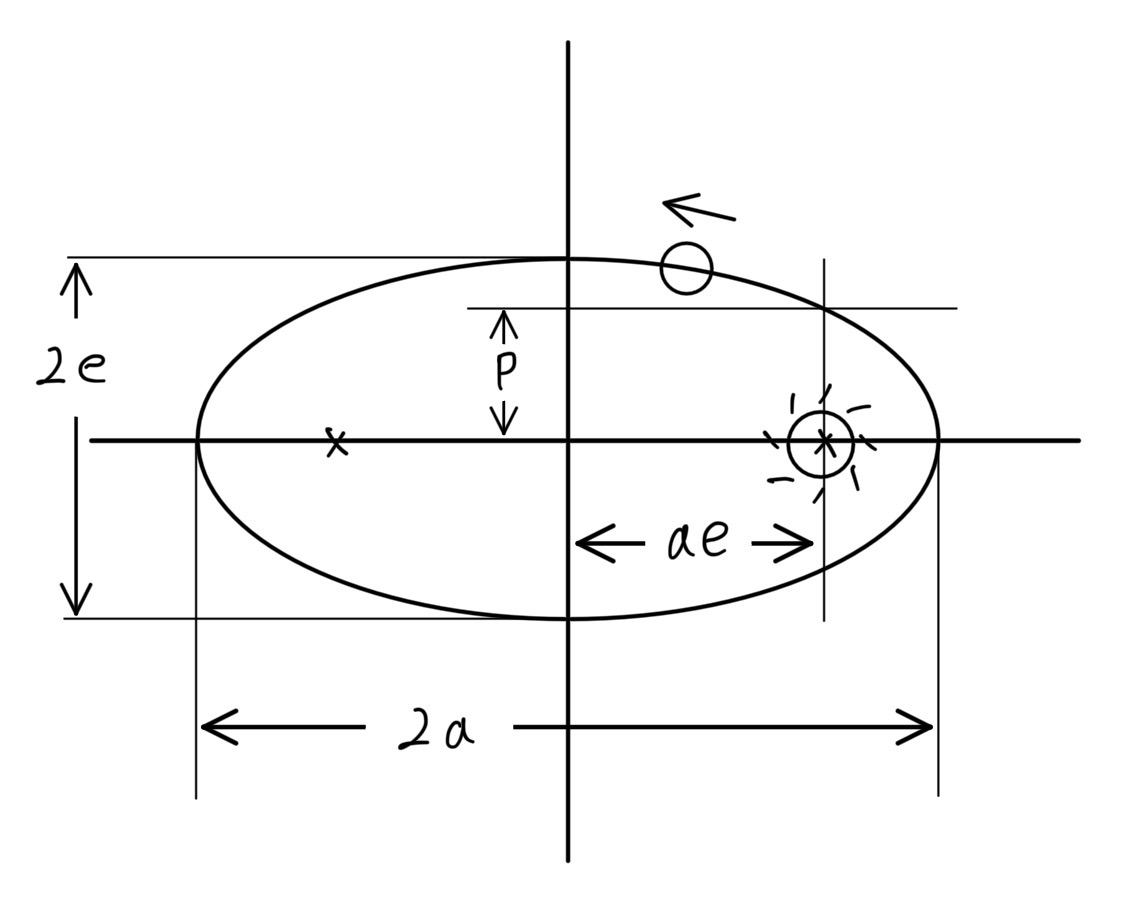
\includegraphics[width=0.9\textwidth]{3.png}
    \caption{Kepler問題：引力の場合、負のエネルギー$E<0$}
    \label{fig:3}
  \end{figure}

  \section{Q2A-6（Kepler問題：引力の場合、正のエネルギー$E>0$）}
  Q2A-5の途中から分岐して、ここではエネルギーが正の場合を考える：
  \begin{align*}
    E>0。\tag{40}
  \end{align*}
  この問題では、\hyperref[fig:4]{図4}を参考にしてください。

  \subsection*{(i)}
  正のエネルギー$E>0$の場合に、軌跡が原点（=力の中心）を焦点とする双曲線になることを示す。Q2A-5で得た軌跡の方程式は次であった：
  \begin{align*}
    r=\frac{p}{1+e\cos\varphi},\qquad p=\frac{l^2}{m\alpha},\qquad e=\sqrt{1+\frac{2El^2}{m\alpha^2}}。
  \end{align*}
  今は$E>0$であるから、離心率に対応する量$e$は：
  \begin{align*}
    e=\sqrt{1+\frac{2El^2}{m\alpha^2}}>1。
  \end{align*}
  次に、この軌跡が双曲線であることを確認する。極座標とDescartes座標の関係$x=r\cos\varphi,\ y=r\sin\varphi$を用いると、軌跡の方程式は：
  \begin{align*}
    r+ex=p。
  \end{align*}
  ここで$r^2=x^2+y^2$であるから、両辺を2乗して整理する：
  \begin{align*}
    x^2+y^2=(p-ex)^2=p^2-2pex+e^2x^2,\qquad \therefore (e^2-1)x^2-y^2-2pex+p^2=0。
  \end{align*}
  これを$x$について平方完成する：
  \begin{align*}
    (e^2-1)\left(x-\frac{pe}{e^2-1}\right)^2-y^2=\frac{p^2}{e^2-1}。
  \end{align*}
  両辺を右辺で割ると：
  \begin{align*}
    \frac{\left(x-\frac{pe}{e^2-1}\right)^2}{\left(\frac{p}{e^2-1}\right)^2}-\frac{y^2}{\frac{p^2}{e^2-1}}=1。
  \end{align*}
  これは双曲線の標準形である。ここで、双曲線とは、2つの焦点からの距離の差の絶対値が一定である点の集合であり、標準形としては：
  \begin{align*}
    \frac{(x-x_0)^2}{a^2}-\frac{y^2}{b^2}=1
  \end{align*}
  の形をもつ曲線である。したがって、$E>0$のとき、軌跡は双曲線であることが示された。

  さらに、この双曲線の焦点を確認する。上で得た標準形より、中心は$\left(\frac{pe}{e^2-1},0\right)$であり、半軸は：
  \begin{align*}
    a=\frac{p}{e^2-1},\qquad b=\frac{p}{\sqrt{e^2-1}}。
  \end{align*}
  双曲線の焦点距離$c$は$c^2=a^2+b^2$で定義されるので：
  \begin{align*}
    c^2=\left(\frac{p}{e^2-1}\right)^2+\frac{p^2}{e^2-1}=\frac{p^2e^2}{(e^2-1)^2},\qquad c=\frac{pe}{e^2-1}。
  \end{align*}
  よって、焦点は：
  \begin{align*}
    \left(\frac{pe}{e^2-1}-c,0\right)=(0,0),\qquad \left(\frac{pe}{e^2-1}+c,0\right)=\left(\frac{2pe}{e^2-1},0\right)。
  \end{align*}
  したがって、原点はこの双曲線の焦点の一つである。以上より、$E>0$のとき軌跡は原点を焦点とする双曲線になることが示された。

  \subsection*{(ii)}
  原点から近日点までの距離$r_{\min}$と、双曲線の半軸$a$を求める。まず、近日点とは、力の中心である原点からの距離$r$が最小となる点である。軌跡の方程式
  \begin{align*}
    r=\frac{p}{1+e\cos\varphi}
  \end{align*}
  において、$e>1$であるから、$r$が最小となるのは分母が最大となる$\cos\varphi=1$のときである。したがって：
  \begin{align*}
    r_{\min}=\frac{p}{e+1}。
  \end{align*}
  次に、双曲線の標準形から半軸$a$を読むと：
  \begin{align*}
    a=\frac{p}{e^2-1}。
  \end{align*}
  これを用いると：
  \begin{align*}
    a(e-1)=\frac{p}{e^2-1}(e-1)=\frac{p}{e+1}=r_{\min}。
  \end{align*}
  したがって：
  \begin{align*}
    r_{\min}=\frac{p}{e+1}=a(e-1)。
  \end{align*}
  最後に、$a$をエネルギー$E$で表す。$e^2=1+\frac{2El^2}{m\alpha^2}$より：
  \begin{align*}
    e^2-1=\frac{2El^2}{m\alpha^2}。
  \end{align*}
  また、$p=\frac{l^2}{m\alpha}$であるから：
  \begin{align*}
    a=\frac{p}{e^2-1}=\frac{\frac{l^2}{m\alpha}}{\frac{2El^2}{m\alpha^2}}=\frac{\alpha}{2E}。
  \end{align*}
  以上より、原点から近日点までの距離$r_{\min}$と双曲線の半軸$a$は次のように与えられる：
  \begin{align*}
    r_{\min}&=\frac{p}{e+1}=a(e-1),\tag{41}\\
    a&=\frac{p}{e^2-1}=\frac{\alpha}{2E}\tag{42}。
  \end{align*}

  \begin{figure}[H]
    \centering
    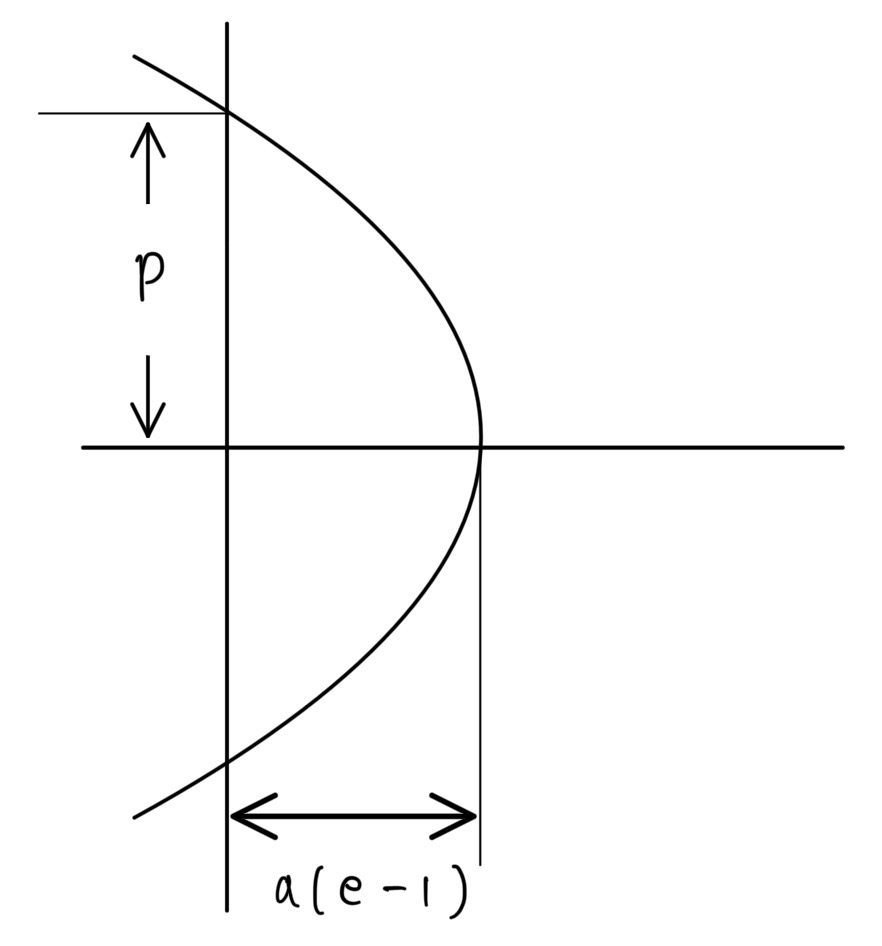
\includegraphics[width=0.6\textwidth]{4.png}
    \caption{Kepler問題：引力の場合、正のエネルギー$E>0$}
    \label{fig:4}
  \end{figure}

  \section{Q2A-7（Kepler問題：引力の場合、ゼロのエネルギー$E=0$）}
  Q2A-5の途中から分岐して、ここではエネルギーがゼロの場合を考える：
  \begin{align*}
    E=0。\tag{43}
  \end{align*}

  \subsection*{(i)}
  ここでは、エネルギー$E=0$の場合に、軌跡が原点を焦点とする放物線になることを示す。Q2A-5で得た軌跡の方程式は次であった：
  \begin{align*}
    r=\frac{p}{1+e\cos\varphi},\qquad p=\frac{l^2}{m\alpha},\qquad e=\sqrt{1+\frac{2El^2}{m\alpha^2}}。
  \end{align*}
  ここに$E=0$を代入すると、離心率に対応する量$e$は：
  \begin{align*}
    e=\sqrt{1+\frac{2\cdot0\cdot l^2}{m\alpha^2}}=1。
  \end{align*}
  したがって、軌跡の方程式は次のようになる：
  \begin{align*}
    r=\frac{p}{1+\cos\varphi}。
  \end{align*}
  この式が原点を焦点とする放物線を表すことを、Descartes座標に直して確認する。極座標とDescartes座標の関係$x=r\cos\varphi,\ y=r\sin\varphi$を用いると、上式は：
  \begin{align*}
    r+x=p。
  \end{align*}
  ここで$r^2=x^2+y^2$であるから、両辺を2乗して整理する：
  \begin{align*}
    x^2+y^2=(p-x)^2=p^2-2px+x^2,\qquad \therefore y^2=-2p\left(x-\frac{p}{2}\right)。
  \end{align*}
  これは$x$軸方向に開く放物線の標準形である。放物線とは、一つの定点である焦点と一つの定直線である準線からの距離が等しい点の集合である。標準形
  \begin{align*}
    y^2=-4a(x-h)
  \end{align*}
  の放物線は、頂点$(h,0)$、焦点$(h-a,0)$、準線$x=h+a$をもつ。今の場合は$h=\frac p2,\ a=\frac p2$であるから、焦点は：
  \begin{align*}
    \left(\frac{p}{2}-\frac{p}{2},0\right)=(0,0)
  \end{align*}
  である。したがって、$E=0$のとき、軌跡は原点を焦点とする放物線になることが示された。

  \subsection*{(ii)}
  ここでは、原点から近日点までの距離$r_{\min}$を求める。近日点とは、力の中心である原点からの距離$r$が最小となる軌道上の点である。今の場合、軌跡の方程式は
  \begin{align*}
    r=\frac{p}{1+\cos\varphi}
  \end{align*}
  である。$r$が最小となるのは、分母$1+\cos\varphi$が最大となるときである。したがって、$\cos\varphi=1$、すなわち$\varphi=0$のときに$r$は最小となる。よって：
  \begin{align*}
    r_{\min}=\frac{p}{1+1}=\frac{p}{2}。\tag{44}
  \end{align*}
  以上より、エネルギー$E=0$の場合、原点から近日点までの距離は$r_{\min}=\frac p2$であることが示された。

  \clearpage
  \part{Kepler問題の補足、その1：動径座標$r$と時間$t$の関係}
  Kepler問題とは、$r^{-1}$に比例するポテンシャル中の1粒子の運動の問題だった。直前のIII部では、Kepler問題のうちで軌跡を求める部分を解いた。つまり、動径座標$r$と角度座標$\varphi$の関数関係を決定した。このIV部では、補足として、Kepler問題のうちで軌道の情報を付け加える。つまり、動径座標$r$と時間$t$の関数関係を決定する。

  \section{Q2A-8（Kepler問題の補足：動径座標$r$と時間$t$の関数関係：引力の場合、負のエネルギー$E<0$）}
  (23)式で与えられるポテンシャルの中での1粒子の運動の考察を続ける。再び、エネルギー$E$が負の場合を考える：
  \begin{align*}
    E<0。\tag{45}
  \end{align*}
  Q2A-5での解析により、粒子の軌跡は楕円になる。以下では、この楕円上の運動での動径座標$t$と時間$t$の関数関係を明らかにする：
  \subsection*{(i)}
  一般論による動径座標$r$と時間$t$の関係は(20)式で与えられている。今の場合にこの式を整理する。\\
  まず$e=\sqrt{1+\frac{2El^2}{m\alpha^2}}\therefore E=\frac{m\alpha^2}{2l^2}(e^2-1)$を代入する：
  \begin{align*}
    t=\int \frac{dr}{\sqrt{\frac{2}{m} \left\{\frac{m\alpha^2}{2l^2}(e^2-1)+\frac{\alpha}{r}\right\}-\frac{l^2}{m^2r^2}}}+(定数)。
  \end{align*}
  被積分関数の分母分子に$r$を掛ける：
  \begin{align*}
    t&=\int \frac{rdr}{\sqrt{\frac{2}{m} \left\{\frac{m\alpha^2}{2l^2}r^2(e^2-1)+\alpha r\right\}-\frac{l^2}{m^2}}}+(定数)\\
    &=\sqrt{\frac{ma}{\alpha}}\int \frac{rdr}{\sqrt{\frac{2a}{\alpha}\left\{\frac{m\alpha^2}{2l^2}r^2(e^2-1)+\alpha r\right\}-\frac{al^2}{\alpha m}}}+(定数)。
  \end{align*}
  ここに楕円における長半径$a=\frac{p}{1-e^2}=\frac{l^2}{(1-e^2)m\alpha}$を用いることで、最終的に次のように整理される：
  \begin{align*}
    t&=\sqrt{\frac{ma}{\alpha}}\int \frac{rdr}{\sqrt{-r^2+2ar-a^2(1-e^2)}}+(定数)\\
    &=\sqrt{\frac{ma}{\alpha}}\int \frac{rdr}{\sqrt{a^2e^2-(r-a)^2}}+(定数)。\tag{46}
  \end{align*}

  \subsection*{(ii)}
  (46)式右辺の積分を評価するために、動径座標$r$をパラメータ$\xi$を用いて、次のように表す：
  \begin{align*}
    r=a(1-e\cos\xi)。\tag{47}
  \end{align*}
  このもとで、(46)式で時間$t$を計算する。まず、これを(46)式に代入する：
  \begin{align*}
    t&=\sqrt{\frac{ma}{\alpha}}\int \frac{a(1-e\cos\xi)ae\sin\xi d\xi}{\sqrt{a^2e^2-(a(1-e\cos\xi)-a)^2}}+(定数)\\
    &=\sqrt{\frac{ma}{\alpha}}\int \frac{a(1-e\cos\xi)ae\sin\xi d\xi}{\sqrt{a^2e^2-(-ae\cos\xi)^2 }}+(定数)\\
    &=\sqrt{\frac{ma}{\alpha}}\int \frac{a(1-e\cos\xi)ae\sin\xi d\xi}{ae\sin\xi}+(定数)\\
    &=\sqrt{\frac{ma}{\alpha}}\int a(1-e\cos\xi)d\xi+(定数)\\
    &=\sqrt{\frac{ma^3}{\alpha}}\left(\xi-e\sin\xi\right)+(定数)。
  \end{align*}
  時間$t$の原点を適当に取ることで積分定数を0とすることができる。したがって、(46)式は次のようになる：
  \begin{align*}
    t=\sqrt{\frac{ma^3}{\alpha}}\left(\xi-e\sin\xi\right)。\tag{48}
  \end{align*}

  \section{Q2A-9（Kepler問題の補足：動径座標$r$と時間$t$の関数関係：引力の場合、正のエネルギー$E>0$）}
  Q2A-8と同様の解析を、今度は、エネルギー$E$が正の場合で行う：
  \begin{align*}
    E>0。\tag{49}
  \end{align*}
  Q2A-6での解析により、粒子の軌跡は双曲線になる。まず双曲線であることから、双曲線関数を用いて表示することを考える。この双曲線上では、動径座標$r$の動く範囲は$r_{\min}=a(e-1)\leq r$である。ゆえに、次のように表示するのが適当だろう：
  \begin{align*}
    r=a(e\cosh\xi-1)。\tag{50}
  \end{align*}
  ここで、双曲線における半軸は$\frac{p}{e^2-1}$であるから、楕円における長半径と符号が反転する。よって(46)式をそのまま使うことはできないため、(20)式を整理し直す：
  \begin{align*}
    t = \int \frac{dr}{\sqrt{\frac2m\left(E-V(r)\right)-\frac{l^2}{m^2r^2}}} + (定数)。
  \end{align*}
  ここに$e=\sqrt{1+\frac{2El^2}{m\alpha^2}}\therefore E=\frac{m\alpha^2}{2l^2}(e^2-1)$を代入する：
  \begin{align*}
    t=\int \frac{dr}{\sqrt{\frac{2}{m} \left\{\frac{m\alpha^2}{2l^2}(e^2-1)+\frac{\alpha}{r}\right\}-\frac{l^2}{m^2r^2}}}+(定数)。
  \end{align*}
  被積分関数の分母分子に$r$を掛ける：
  \begin{align*}
    t=\int \frac{rdr}{\sqrt{\frac{2}{m} \left\{\frac{m\alpha^2}{2l^2}(e^2-1)r^2+\alpha r\right\}-\frac{l^2}{m^2}}}+(定数)\\
    =\sqrt{\frac{ma}{\alpha}}\int \frac{rdr}{\sqrt{\frac{2a}{\alpha}\left\{\frac{m\alpha^2}{2l^2}(e^2-1)r^2+\alpha r\right\}-\frac{al^2}{\alpha m}}}+(定数)。
  \end{align*}
  ここに双曲線における半軸$a=\frac{p}{e^2-1}=\frac{l^2}{(e^2-1)m\alpha}$を用いることで、最終的に次のように整理される：
  \begin{align*}
    t=\sqrt{\frac{ma}{\alpha}}\int \frac{rdr}{\sqrt{(r+a)^2-a^2e^2}}+(定数)。\tag*{(46)'}
  \end{align*}
  ここで、(50)式を(46)'式に代入する：
  \begin{align*}
    t=\sqrt{\frac{ma}{\alpha}}\int \frac{a(e\cosh\xi-1)ae\sinh\xi d\xi}{\sqrt{(a(e\cosh\xi-1)+a)^2-a^2e^2}}+(定数)\\
    =\sqrt{\frac{ma}{\alpha}}\int \frac{a(e\cosh\xi-1)ae\sinh\xi d\xi}{\sqrt{(ae\cosh\xi)^2-a^2e^2}}+(定数)\\
    =\sqrt{\frac{ma}{\alpha}}\int \frac{a(e\cosh\xi-1)ae\sinh\xi d\xi}{ae\sinh\xi}+(定数)\\
    =\sqrt{\frac{ma}{\alpha}}\int a(e\cosh\xi-1)d\xi+(定数)\\
    =\sqrt{\frac{ma^3}{\alpha}}\left(e\sinh\xi-\xi\right)+(定数)。
  \end{align*}
  時間$t$の原点を適当に取ることで積分定数を0とすることができる。したがって、(46)'式は次のようになる：
  \begin{align*}
    t=\sqrt{\frac{ma^3}{\alpha}}\left(e\sinh\xi-\xi\right)。\tag{51}
  \end{align*}

  \part{Kepler問題の補足、その2：Runge-Lentzベクトル$A$}

  \section{Q2A-10（Runge-Lentzベクトル$A$）}
  (23)式で与えられた$r^-1$に比例する中心力ポテンシャルの中での1粒子の運動の解析を続ける。\\
  粒子の座標ベクトル$\vect{r}$、速度ベクトル$\vect{v}=\dot{\vect{r}}$、角運動量ベクトル$\vect{l}=m\vect{r}\times\vect{v}$を用いて、Runge-Lentzベクトル$\vect{A}$を次のように定義する：
  \begin{align*}
    \vect{A}=\vect{v}\times\vect{l}-\alpha\frac{\vect{r}}{|\vect{r}|}。\tag{52}
  \end{align*}
  
  \subsection*{(i)}
  (23)式で与えられた、$r^{-1}$に比例する中心力ポテンシャルの中でのKepler運動においては、Runge-Lentzベクトル$\vect{A}$が運動の定数になることを示す：
  \begin{align*}
    \bbn{\vect{A}}{t}=0。\tag{53}
  \end{align*}
  $r=|\vect{r}|$とする。まず、ポテンシャル$V(r)=-\alpha/r$から力を求める。力は$\vect{F}=-\nabla V$であるから、
  \begin{align*}
    m\dot{\vect{v}}=\vect{F}=-\frac{\alpha}{r^3}\vect{r}。
  \end{align*}
  この力は常に$\vect{r}$に平行であるため、角運動量は保存する：
  \begin{align*}
    \bbn{\vect{l}}{t}=m\vect{r}\times\dot{\vect{v}}=\vect{0}。
  \end{align*}
  したがって、$\vect{A}$の時間微分は次のように書ける：
  \begin{align*}
    \bbn{\vect{A}}{t}=\dot{\vect{v}}\times\vect{l}-\alpha\bbn{}{t}\left(\frac{\vect{r}}{r}\right)。
  \end{align*}
  ここで、まず第1項を計算する。$\dot{\vect{v}}=-\alpha\vect{r}/(mr^3)$と$\vect{l}=m\vect{r}\times\vect{v}$を代入し、ベクトル三重積の公式$\vect{a}\times(\vect{b}\times\vect{c})=(\vect{a}\cdot\vect{c})\vect{b}-(\vect{a}\cdot\vect{b})\vect{c}$を用いる：
  \begin{align*}
    \dot{\vect{v}}\times\vect{l}=-\frac{\alpha}{r^3}\vect{r}\times(\vect{r}\times\vect{v})=-\frac{\alpha}{r^3}\{(\vect{r}\cdot\vect{v})\vect{r}-r^2\vect{v}\}=\alpha\left(\frac{\vect{v}}{r}-\frac{(\vect{r}\cdot\vect{v})\vect{r}}{r^3}\right)。
  \end{align*}
  一方、単位ベクトル$\vect{r}/r$の時間微分は,
  \begin{align*}
    \bbn{}{t}\left(\frac{\vect{r}}{r}\right)=\frac{\vect{v}}{r}-\frac{(\vect{r}\cdot\vect{v})\vect{r}}{r^3}。
  \end{align*}
  よって、これらを$\bbn{\vect{A}}{t}$に代入する：
  \begin{align*}
    \bbn{\vect{A}}{t}=\alpha\left(\frac{\vect{v}}{r}-\frac{(\vect{r}\cdot\vect{v})\vect{r}}{r^3}\right)-\alpha\left(\frac{\vect{v}}{r}-\frac{(\vect{r}\cdot\vect{v})\vect{r}}{r^3}\right)=\vect{0}。
  \end{align*}
  以上より、Runge-Lentzベクトル$\vect{A}$が運動の定数になることが示された。
  
  \subsection*{(ii)}
  本小問では、Runge-Lentzベクトル$\vect{A}$の幾何学的意味を調べる。まず、$\vect{A}$と位置ベクトル$\vect{r}$の内積を計算する。定義式に$\vect{r}$を内積する：
  \begin{align*}
    \vect{A}\cdot\vect{r}=(\vect{v}\times\vect{l})\cdot\vect{r}-\alpha r。
  \end{align*}
  ここで、スカラー三重積の巡回性$(\vect{v}\times\vect{l})\cdot\vect{r}=\vect{l}\cdot(\vect{r}\times\vect{v})$を用いる。また、$\vect{l}=m\vect{r}\times\vect{v}$であるから、$\vect{r}\times\vect{v}=\vect{l}/m$である。したがって：
  \begin{align*}
    \vect{A}\cdot\vect{r}=\vect{l}\cdot\frac{\vect{l}}{m}-\alpha r=\frac{l^2}{m}-\alpha r。
  \end{align*}
  ここで、$\vect{A}$と$\vect{r}$のなす角を$\psi$とすると、$\vect{A}\cdot\vect{r}=|\vect{A}|r\cos\psi$である。よって：
  \begin{align*}
    |\vect{A}|r\cos\psi=\frac{l^2}{m}-\alpha r。
  \end{align*}
  これを$r$について解く：
  \begin{align*}
    r=\frac{l^2/(m\alpha)}{1+\frac{|\vect{A}|}{\alpha}\cos\psi}。
  \end{align*}
  一方、Q2A-5で得たKepler軌道の方程式は：
  \begin{align*}
    r=\frac{p}{1+e\cos\varphi},\qquad p=\frac{l^2}{m\alpha}。
  \end{align*}
  したがって、$\vect{A}$の方向を$\varphi=0$の方向として角度を測れば、上の式はKepler軌道の式と一致する。このとき、$\psi=0$で分母が最大となり、$r$は最小となる。すなわち、$\vect{A}$の方向は原点から見た近日点の方向である。ただし、$|\vect{A}|=0$の場合は円軌道であり、近日点の方向は一意に定まらない。
  
  さらに、両者の軌道方程式を比較すると、離心率$e$は次のように読める：
  \begin{align*}
    e=\frac{|\vect{A}|}{\alpha}。
  \end{align*}
  したがって、Runge-Lentzベクトルの大きさは離心率に比例し、
  \begin{align*}
    |\vect{A}|=\alpha e\tag{54}
  \end{align*}
  が成り立つ。以上より、Runge-Lentzベクトル$\vect{A}$の方向は近日点方向を表し、その大きさは離心率$e$に比例することが示された。
  
  \part{微小振動：定式化}

  \section{Q2A-11（自由度$f$の古典力学系の安定な固定点のまわりの微小振動を表すLagrange関数）}
  自由度$f$の古典力学系が安定な固定点を持つとする。

  \subsection*{(i)}
  「安定な固定点」とは何か。\\
  まず単に「固定点」といった場合、それは停留点、つまりポテンシャルエネルギー$V(q_1,q_2,\dots,q_f)$の勾配が$\vect{0}$となる点である。\\
  次に「安定な固定点」とは、停留点の中でもポテンシャルエネルギーが極小値を取る点である。

  以降、一般座標$q_1,q_2,\dots,q_f$を、安定な固定点が原点となるように用意する。つまり、$(q_1,q_2,\dots,q_f)=(0,0,\dots,0)$が固定点である。
  
  \subsection*{(ii)}
  安定な固定点の周りの振幅が十分小さな振動を考える。このとき、この系のLagrange関数$L$は、$q_i$の振幅が小さいとして展開して、意味のない定数を捨てて、さらに、展開の高次の項を無視すると、次の形をとることを示す：
  \begin{align*}
    L=\frac12 \left(\dot{\vect{q}}^t M\dot{\vect{q}}-\vect{q}^t N\vect{q}\right)。\tag{55}
  \end{align*}
  ただし、$\vect{q}$は一般座標$q_1,q_2,\dots,q_f$を並べた列ベクトルである：
  \begin{align*}
    \vect{q}=
    \begin{bmatrix}
      q_1\,q_2\,\cdots\,q_f
    \end{bmatrix}^t。\tag{56}
  \end{align*}
  また、$M$と$N$は実定数を要素とする$f$次対称行列である。\\
  まず、運動エネルギーは各自由度に対して次のように書ける：
  \begin{align*}
    T_i=\frac{1}{2}m_i\dot{\vect{q}}_i^2\quad(i=1,2,\dots,f)。
  \end{align*}
  ここで、$M$を$M_{ii}=m_i$である実対角行列として導入すると、運動エネルギーの和$T$は次のように書ける：
  \begin{align*}
    T=\frac12 \dot{\vect{q}}^t M\dot{\vect{q}}。
  \end{align*}
  次に、ポテンシャルエネルギー$V(\vect{q})$を固定点$\vect{q}=\vect{0}$のまわりでTaylor展開する：
  \begin{align*}
    V(\vect{q})=V(\vect{0})+\sum_{i}\left\{q_i\hb{V}{q_i}(0,0)\right\}+\frac12 \sum_{i,j}\left\{q_iq_j \frac{\partial^2 V}{\partial q_i \partial q_j}(0,0)\right\}。
  \end{align*}
  定数項はLagrange関数に意味のある寄与をしないので捨てる。また、固定点ではポテンシャルエネルギーの勾配が$\vect{0}$であるから、ポテンシャルの1次の項も消える。したがって、3次以降を捨てると、残る項は2次の項である。さらに、$N_{ij}=\frac{\partial^2 V}{\partial q_i \partial q_j}(0,0)$として$N$を導入すると、ポテンシャルエネルギーは次のように書ける：
  \begin{align*}
    V(\vect{q})=\frac{1}{2}\vect{q}^{t}N\vect{q}。
  \end{align*}
  ここで、偏微分は交換可能であるから、$N_{ij}=N_{ji}$である。よって$N$は実対称行列である。以上より、微小振動を記述するLagrange関数は次の形に書ける：
  \begin{align*}
    L=T-V=\frac{1}{2}\left(\dot{\vect{q}}^{t}M\dot{\vect{q}}-\vect{q}^{t}N\vect{q}\right)。
  \end{align*}

  
  \subsection*{(iii)}
  本小問では、安定な固定点のまわりの微小振動において、行列$M$と$N$が正定値であることを説明する。まず、実対称行列$A$が正定値であるとは、任意の非零実ベクトル$\vect{x}$に対して
  \begin{align*}
    \vect{x}^{t}A\vect{x}>0
  \end{align*}
  が成り立つことをいう。運動エネルギーは、非零の速度$\dot{\vect{q}}\neq\vect{0}$に対して正でなければならない。したがって、
  \begin{align*}
    T=\frac{1}{2}\dot{\vect{q}}^{t}M\dot{\vect{q}}>0\qquad(\dot{\vect{q}}\neq\vect{0})
  \end{align*}
  であり、$M$は正定値である。次に、原点が安定な固定点であることは、ポテンシャルエネルギーが原点で局所的な最小値を持つことを意味する。今回、最低次で打ち切った2次形式の段階で安定性が実現されていると仮定しているので、任意の非零変位$\vect{q}\neq\vect{0}$に対して、
  \begin{align*}
    V(\vect{q})=\frac{1}{2}\vect{q}^{t}N\vect{q}>V(\vect{0})=0
  \end{align*}
  が成り立つ。したがって、$N$も正定値である。以上より、微小振動を表すLagrange関数に現れる実対称行列$M,N$はいずれも正定値であることが示された。
  
  \section{Q2A-12（実対称行列の平方根）}
  
  \subsection*{(i)}
  本小問では、実対称行列$A$が直交行列$O$により対角化されているとき、行列$A$の平方根を具体的に書く。\\
  定理1より、$A$は次のように書ける：
  \begin{align*}
    A=O\mathrm{diag}(a_1,a_2,\ldots,a_n)O^{t}。
  \end{align*}
  ここで、$\left\{\mathrm{diag}(\pm\sqrt{a_1},\pm\sqrt{a_2},\ldots,\pm\sqrt{a_n})\right\}^2=\mathrm{diag}(a_1,a_2,\ldots,a_n)$であるから、
  \begin{align*}
    A&=O\mathrm{diag}(a_1,a_2,\ldots,a_n)O^{t}\\
    &=O\left\{\mathrm{diag}(\pm\sqrt{a_1},\pm\sqrt{a_2},\ldots,\pm\sqrt{a_n})\right\}^2O^t\\
    &=O\mathrm{diag}(\pm\sqrt{a_1},\ldots,\pm\sqrt{a_n})\mathrm{diag}(\pm\sqrt{a_1},\ldots,\pm\sqrt{a_n})O^{t}\\
    &=O\mathrm{diag}(\pm\sqrt{a_1},\ldots,\pm\sqrt{a_n})O^{t}O\mathrm{diag}(\pm\sqrt{a_1},\ldots,\pm\sqrt{a_n})O^{t}\\
    &=\left\{O\mathrm{diag}(\pm\sqrt{a_1},\ldots,\pm\sqrt{a_n})O^{t}\right\}^2。
  \end{align*}
  よって$A$の平方根を次のように与えることができる：
  \begin{align*}
    A^{1/2}=O\mathrm{diag}(\pm\sqrt{a_1},\pm\sqrt{a_2},\ldots,\pm\sqrt{a_n})O^{t}。\tag{60}
  \end{align*}
  符号の選び方はそれぞれ独立であるから、$2^n$通りある。
  
  
  \subsection*{(ii)}
  本小問では、(60)式で与えた$A^{1/2}$が実対称行列とは限らないことを説明する。\\
  実対称行列$A$の固有値$a_i$は実数であるが、正であるとは限らない。もし、ある固有値$a_i$が負ならば、$\sqrt{a_i}$は実数ではない。したがって、そのような固有値を含む場合、(60)式に現れる対角行列は複素成分を持つ。よって、(60)式で定義される$A^{1/2}$は一般には実行列とは限らず、したがって実対称行列とも限らない。
  
  \subsection*{(iii)}
  本小問では、$A$が正定値である場合に、$A^{1/2}$の性質を調べる。\\
  $A$が正定値であれば、定理1より、すべての固有値は正である：
  \begin{align*}
    a_i>0\qquad(1\leq i\leq n)。
  \end{align*}
  したがって、$\sqrt{a_i}$はすべて実数である。このとき、(60)式の$A^{1/2}$は実行列であり、さらに
  \begin{align*}
    (A^{1/2})^{t}=(A^t)^{1/2}=A^{1/2}
  \end{align*}
  であるから、実対称行列である。また、$A^{1/2}$が正定値であるためには、その固有値がすべて正であることが必要。したがって、$2^n$通りの符号選択のうち、すべての符号を正に取る1通りだけが正定値の平方根を与える：
  \begin{align*}
    A^{1/2}=O\mathrm{diag}(\sqrt{a_1},\sqrt{a_2},\ldots,\sqrt{a_n})O^{t}。
  \end{align*}
  
  \subsection*{(iv)}
  本小問では、$A^{-1/2}$をどのように表すかを確認する。$A^{-1/2}$が存在するためには、$A^{1/2}$が可逆でなければならない。すなわち、$a_i\neq0$が必要である。この条件のもとで、
  \begin{align*}
    A^{-1/2}=O\mathrm{diag}\left(\frac{1}{\pm\sqrt{a_1}},\frac{1}{\pm\sqrt{a_2}},\ldots,\frac{1}{\pm\sqrt{a_n}}\right)O^{t}
  \end{align*}
  と書ける。実際、この行列を$A^{1/2}$に掛けると単位行列が得られる：
  \begin{align*}
    A^{1/2}A^{-1/2}=OO^{t}=I。
  \end{align*}
  
  \subsection*{(v)}
  本小問では、$A$が正定値の場合に、$A^{-1/2}$も実対称行列であり、さらに正定値となることを示す。\\
  $A$が正定値ならば$a_i>0$であるから、$\frac{1}{\sqrt{a_i}}$は実数である。よって、$A^{-1/2}$は実行列である。さらに
  \begin{align*}
    (A^{-1/2})^{t}=(A^{t})^{-1/2}=A^{-1/2}
  \end{align*}
  であるから、実対称行列である。\\
  また、$A^{1/2}$が正定値であるとき、任意の非零実ベクトル$\vect{y}$に対して、$\vect{y}=A^{1/2}\vect{x}$と書くと、
  \begin{align*}
    \vect{y}^tA^{-1/2}\vect{y}=(A^{1/2}\vect{x})^t \vect{x}=\vect{x}^tA^{1/2}\vect{x}>0。
  \end{align*}
  よってこのとき、$A^{-1/2}$も正定値である。
  
  \section{Q2A-13（基準振動：基本）}
  Q2A-11の設定を引き継ぐ。自由度$f$の微小振動を表すLagrange関数$L$は(55)式で与えられている。この問題では、Lagrange関数$L$において、古い一般座標$q_1,q_2,\dots,q_f$を新しい一般座標$Q_1,Q_2,\dots,Q_f$へうまく一般座標変換して、新しい一般座標$Q_i(1\leq i\leq f)$のひとつひとつが独立な振動を表すようにする。
  \subsection*{(i)}
  本小問では、微小振動を表すLagrange関数を、行列$M^{1/2}$を用いて書き換える。出発点は
  \begin{align*}
    L=\frac{1}{2}\left(\dot{\vect{q}}^{t}M\dot{\vect{q}}-\vect{q}^{t}N\vect{q}\right)
  \end{align*}
  である。\\
  $M$は正定値実対称行列であるから、Q2A-12より、正定値実対称な$M^{1/2}$と$M^{-1/2}$を取ることができる。まず、運動エネルギーの項については、
  \begin{align*}
    \dot{\vect{q}}^{t}M\dot{\vect{q}}=\dot{\vect{q}}^tM^{1/2}M^{1/2}\dot{\vect{q}}=(M^{1/2}\dot{\vect{q}})^t M^{1/2}\dot{\vect{q}}=\left(\bbn{}{t}(M^{1/2}\vect{q})\right)^{t}\bbn{}{t}(M^{1/2}\vect{q})。
  \end{align*}
  また、ポテンシャルの項は、
  \begin{align*}
    \vect{q}^{t}N\vect{q}=\vect{q}^tM^{1/2} M^{-1/2}NM^{-1/2}M^{1/2}\vect{q}=(M^{1/2}\vect{q})^{t}M^{-1/2}NM^{-1/2}(M^{1/2}\vect{q})。
  \end{align*}
  したがって、Lagrange関数は次のように書き換えられる：
  \begin{align*}
    L=\frac{1}{2}\left\{\left(\bbn{}{t}(M^{1/2}\vect{q})\right)^{t}\bbn{}{t}(M^{1/2}\vect{q})-(M^{1/2}\vect{q})^{t}(M^{-1/2}NM^{-1/2})(M^{1/2}\vect{q})\right\}。\tag{61}
  \end{align*}
  
  \subsection*{(ii)}
  本小問では、行列$M^{-1/2}NM^{-1/2}$が実対称行列であり、かつ正定値であることを示す。\\
  まず、$M^{-1/2}$と$N$はいずれも実対称行列であるから、
  \begin{align*}
    (M^{-1/2}NM^{-1/2})^{t}=M^{-1/2}NM^{-1/2}
  \end{align*}
  である。したがって、この行列は実対称行列である。次に、任意の非零実ベクトル$\vect{x}$に対して、
  \begin{align*}
    \vect{x}^{t}M^{-1/2}NM^{-1/2}\vect{x}=(M^{-1/2}\vect{x})^{t}N(M^{-1/2}\vect{x})
  \end{align*}
  が成り立つ。$M^{-1/2}$は可逆であるから、$\vect{x}\neq\vect{0}$ならば$M^{-1/2}\vect{x}\neq\vect{0}$である。また、$N$は正定値である。よって、
  \begin{align*}
    (M^{-1/2}\vect{x})^{t}N(M^{-1/2}\vect{x})>0
  \end{align*}
  である。したがって、$M^{-1/2}NM^{-1/2}$は正定値であることが示された。
  
  \subsection*{(iii)}
  本小問では、行列$M^{-1/2}NM^{-1/2}$を直交行列により対角化する。\\
  前小問より、この行列は正定値実対称行列である。したがって、定理1より、ある直交行列$O$が存在して、
  \begin{align*}
    M^{-1/2}NM^{-1/2}=O\mathrm{diag}(a_1,a_2,\ldots,a_f)O^{t}
  \end{align*}
  と書ける。また、この行列は正定値であるから固有値はすべて正である。したがって、各固有値の平方根は実数である。よって$\omega_i=\sqrt{a_i}$と取ると、次のように表すことができる：
  \begin{align*}
    M^{-1/2}NM^{-1/2}=O\mathrm{diag}(\omega_1^2,\omega_2^2,\ldots,\omega_f^2)O^{t}。\tag{62}
  \end{align*}
  ただし、$O$は直交行列である：
  \begin{align*}
    O^t=O^{-1}。\tag{63}
  \end{align*}
  また、$\omega_i$はすべて正である：
  \begin{align*}
    \omega_1,\omega_2,\dots,\omega_f>0。\tag{64}
  \end{align*}
  
  
  \subsection*{(iv)}
  新しい一般座標$Q_1,Q_2,\dots,Q_f$の列ベクトル$\vect{Q}$を次のように定める：
  \begin{align*}
    \vect{Q}=\begin{bmatrix}Q_1&Q_2&\cdots&Q_f\end{bmatrix}^{t}=O^{t}M^{1/2}\vect{q}。\tag{65}
  \end{align*}
  この定義より、$M^{1/2}\vect{q}=O\vect{Q}$である。これを(61)式に代入する：
  \begin{align*}
    L&=\frac{1}{2}\left(\dot{\vect{Q}}^{t}O^{t}O\dot{\vect{Q}}-\vect{Q}^{t}O^{t}M^{-1/2}NM^{-1/2}O\vect{Q}\right) \\
     &=\frac{1}{2}\left(\dot{\vect{Q}}^{t}\dot{\vect{Q}}-\vect{Q}^{t}\mathrm{diag}(\omega_1^2,\omega_2^2,\ldots,\omega_f^2)\vect{Q}\right) \\
     &=\frac{1}{2}\ssum{i}{1}{f}\left(\dot{Q}_i^2-\omega_i^2Q_i^2\right)。\tag{66}
  \end{align*}
  
  \subsection*{(v)}
  本小問では、新しい一般座標$Q_i$に対するEuler-Lagrange方程式を求める。(66)式より、
  \begin{align*}
    \hb{L}{\dot{Q}_i}=\dot{Q}_i,\qquad \hb{L}{Q_i}=-\omega_i^2Q_i
  \end{align*}
  である。Euler-Lagrange方程式$\bbn{}{t}\left(\hb{L}{\dot{Q}_i}\right)=\hb{L}{Q_i}$に代入する：
  \begin{align*}
    \ddot{Q}_i+\omega_i^2Q_i=0\qquad(1\leq i\leq f)。\tag{67}
  \end{align*}
  したがって、各$Q_i$は角振動数$\omega_i$をもつ調和振動を独立に行う。
  
  \subsection*{(vi)}
  本小問では、新しい一般座標$Q_i$による一般解を書き下す。\\
  (67)式は1次元の単振動の方程式であるから、各$i$について一般解は次のように書ける：
  \begin{align*}
    Q_i(t)=A_i\cos(\omega_i t+\theta_i)\qquad(1\leq i\leq f)。\tag{68}
  \end{align*}
  ここで、$A_i$と$\theta_i$は任意定数である。したがって、$f$個の基準座標に対して合計$2f$個の任意定数が現れ、これは自由度$f$の2階常微分方程式系の一般解として必要な個数と一致している。
  
  \subsection*{(vii)}
  本小問では、「$Q_1,Q_2,\ldots,Q_f$が独立に振動する」とは何を意味するかを説明する。(66)式で得たLagrange関数は、
  \begin{align*}
    L=\frac{1}{2}\ssum{i}{1}{f}\left(\dot{Q}_i^2-\omega_i^2Q_i^2\right)
  \end{align*}
  であり、異なる$i$と$j$が混合した項を含まない。したがって、運動方程式も
  \begin{align*}
    \ddot{Q}_i+\omega_i^2Q_i=0
  \end{align*}
  のように、各$i$について閉じた方程式になる。すなわち、ある$Q_i$の運動は他の$Q_j$に影響されず、各基準座標の振幅と位相を独立に選ぶことができる。この意味で、$Q_1,Q_2,\ldots,Q_f$は独立に振動している。これらの$Q_i$を基準座標、各$Q_i$の調和振動を基準振動という。
  
  \subsection*{(viii)}
  本小問では、古い一般座標$\vect{q}$を基準座標$\vect{Q}$で表す。定義(65)式より、
  \begin{align*}
    \vect{Q}=O^{t}M^{1/2}\vect{q}
  \end{align*}
  である。両辺に左から$O$を掛けると、$O\vect{Q}=M^{1/2}\vect{q}$である。さらに左から$M^{-1/2}$を掛ける：
  \begin{align*}
    \vect{q}=M^{-1/2}O\vect{Q}。\tag{69}
  \end{align*}
  
  \subsection*{(ix)}
  本小問では、基準座標ベクトル$\vect{Q}$を標準基底で展開する。$i$番目の標準基底ベクトル$\vect{e}_i$を、
  \begin{align*}
    \vect{e}_i=\begin{bmatrix}0&\cdots&0&1&0&\cdots&0\end{bmatrix}^{t}\qquad(1\leq i\leq f)
  \end{align*}
  と定める。ここで、成分$1$は$i$番目の位置にある。このとき、任意の$\vect{Q}$は標準基底により次のように展開できる：
  \begin{align*}
    \vect{Q}=\ssum{i}{1}{f}Q_i\vect{e}_i。\tag{71}
  \end{align*}
  
  \subsection*{(x)}
  各$i$に対して、ベクトル$\vect{q}_i$を次のように定める。
  \begin{align*}
    \vect{q}_i=M^{-1/2}O\vect{e}_i\qquad(1\leq i\leq f)。\tag{72}
  \end{align*}
  この$\vect{q}_i$は時間によらない定数ベクトルである。(69)式と(71)式を用いると、古い一般座標$\vect{q}$は次のように表せる：
  \begin{align*}
    \vect{q}(t)=M^{-1/2}O\ssum{i}{1}{f}Q_i(t)\vect{e}_i=\ssum{i}{1}{f}Q_i(t)\vect{q}_i。\tag{73}
  \end{align*}

  \subsection*{(xi)}
  本小問では、$\vect{q}_i$が表す意味を説明する。前小問で得た
  \begin{align*}
    \vect{q}(t)=\ssum{i}{1}{f}Q_i(t)\vect{q}_i
  \end{align*}
  より、$i$番目の基準振動だけを考えた場合、すなわち$Q_i(t)$だけが非零で他の$Q_j(t)(j\neq i)$がすべて0である場合には、
  \begin{align*}
    \vect{q}(t)=Q_i(t)\vect{q}_i
  \end{align*}
  となる。したがって、$\vect{q}_i$は、$i$番目の基準振動において古い一般座標$q_1,\ldots,q_f$がどの相対比で振動するかを表している。よって、$\vect{q}_i$は「$i$番目の基準振動の古い一般座標での振幅ベクトル」である。
  
  \subsection*{(xii)}
  本小問では、基準振動の振幅ベクトル$\vect{q}_i$が、$M$を重みとする内積に関して正規直交することを示す。定義より、
  \begin{align*}
    \vect{q}_i=M^{-1/2}O\vect{e}_i,\qquad \vect{q}_j=M^{-1/2}O\vect{e}_j。
  \end{align*}
  したがって、
  \begin{align*}
    \vect{q}_i^{t}M\vect{q}_j=\vect{e}_i^{t}O^{t}M^{-1/2}MM^{-1/2}O\vect{e}_j=\vect{e}_i^{t}O^{t}O\vect{e}_j=\vect{e}_i^{t}\vect{e}_j=\delta_{ij}。
  \end{align*}
  以上より、
  \begin{align*}
    \vect{q}_i^{t}M\vect{q}_j=\delta_{ij}\qquad(1\leq i,j\leq f)\tag{74}
  \end{align*}
  が示された。

  \section{Q2A-14（基準振動：補足）}
  Q2A-13の設定を引き継ぐ。
  \subsection*{(i)}
  本小問では、Q2A-13で得た基準振動の角振動数が、行列式を用いた代数方程式から決まることを示す。\\
  微小振動のLagrange関数は、
  \begin{align*}
    L=\frac{1}{2}\left(\dot{\vect{q}}^{t}M\dot{\vect{q}}-\vect{q}^{t}N\vect{q}\right)。
  \end{align*}
  Euler-Lagrange方程式を各成分について書けば、行列形式で次が成り立つ：
  \begin{align*}
    M\ddot{\vect{q}}+N\vect{q}=\vect{0}。
  \end{align*}
  基準振動では、$\sum_i \vect{q}_iA_i\cos(\omega_i t+\theta_i)$で振動する。各$i$について上の運動方程式を満たすため、$\vect{q}(t)=\vect{q}_i\cos(\omega_i t+\theta_i)$を代入する（$A_i$は共通因数として払われるため、はじめから1とする。）：
  \begin{align*}
    -\omega_i^2M\vect{q}_i+N\vect{q}_i=\vect{0}。
  \end{align*}
  したがって、基準振動の振幅ベクトル$\vect{q}_i$は次を満たす：
  \begin{align*}
    (N-\omega_i^2M)\vect{q}_i=\vect{0}。
  \end{align*}
  非自明な振幅ベクトル$\vect{q}_i\neq\vect{0}$が存在するためには、係数行列の行列式が0でなければならない。よって、次の式を満たす：
  \begin{align*}
    \det(N-\omega_i^2M)=0\qquad(1\leq i\leq f)。\tag{75}
  \end{align*}
  これがまさに$\omega_i$を決定する方程式である。
  
  \subsection*{(ii)}
  前小問において、すでに次の式が得られている：
  \begin{align*}
    (N-\omega_i^2M)\vect{q}_i=\vect{0}。\tag{76}
  \end{align*}
  これが、$\vect{q}_i$の満たす方程式である。この方程式が解を持つとき、全体の比例因子は定まらないが、それを除けば解として$\vect{q}_i$を決定することができる。
  
  \subsection*{(iii)}
  本小問では、振幅ベクトルの全体の比例因子を、規格化条件により定める。\\
  Q2A-13の設定のもとでは、(74)式より、$\vect{q}_i$は$M$を重みとする内積に関して正規直交する。特に、$i=j$のとき、
  \begin{align*}
    \vect{q}_i^{t}M\vect{q}_i=1。\tag{77}
  \end{align*}
  したがって、この(77)式が、振幅ベクトル全体の比例因子を決定するための規格化条件である。\\

  この節で得られたことを、枠で囲って整理しておく。
  \begin{framed}
    \underline{微小振動系の基準振動}：\\
    自由度$f$の微小振動系のLagrange関数：
    \begin{align*}
      L=\frac12 \left(\dot{q}^tM\dot{q}-q^tNq\right)。\tag{78}
    \end{align*}
    ただし、$M$と$N$は正定値の$f$次実対称行列である。このとき、\\
    基準振動の角振動数$\omega_1,\omega_2,\dots,\omega_f$の方程式：
    \begin{align*}
      \det(N-\omega_i^2M)=0\qquad(1\leq i\leq f)。\tag{79}
    \end{align*}
    基準振動の振幅ベクトル$\vect{q}_1,\vect{q}_2,\dots,\vect{q}_f$の方程式：
    \begin{align*}
      (N-\omega_i^2M)\vect{q}_i=\vect{0}\qquad(1\leq i\leq f)。\tag{80}
    \end{align*}
    基準振動の振幅ベクトル$\vect{q}_1,\vect{q}_2,\dots,\vect{q}_f$の正規直交性：
    \begin{align*}
      \vect{q}_i^tM\vect{q}_j=\delta_{ij}\qquad(1\leq i,j\leq f)。\tag{81}
    \end{align*}
    一般解：
    \begin{align*}
      \vect{q}(t)=\ssum{i}{1}{f}Q_i(t)\vect{q}_i。\tag{82}
    \end{align*}
    基準座標$Q_1,Q_2,\dots,Q_f$の独立な基準振動：
    \begin{align*}
      Q_i(t)=A_i\cos(\omega_i t+\theta_i)\qquad(1\leq i\leq f)。\tag{83}
    \end{align*}
    ここで、$A_1,A_2,\ldots,A_f$と$\theta_1,\theta_2,\ldots,\theta_f$は一般解を表す$2f$個の任意定数である。
  \end{framed}
  
  \part{微小振動：例題、その1：多自由度の振り子}
  \section{Q2A-15（2重振り子の平衡点の周りの微小振動）}
  Q2A-1で考察した2重振り子を取り上げる。
  \subsection*{(i)}
  ポテンシャルエネルギー$V$を確認する。(1)式よりLagrange関数$L$は次であった：
  \begin{align*}
    L =\frac{1}{2}(m_1 + m_2)l_1^2\dot{\varphi}_1^2   + m_2l_1l_2\cos(\varphi_1-\varphi_2)\dot{\varphi_1}\dot{\varphi_2} + \frac{1}{2}m_2l_2^2\dot{\varphi}_2^2 + (m_1 + m_2)gl_1\cos\varphi_1 + m_2gl_2\cos\varphi_2。
  \end{align*}
  よってこのうちポテンシャルエネルギーの項を読むと、
  \begin{align*}
    V=-(m_1+m_2)gl_1\cos\varphi_1-m_2gl_2\cos\varphi_2。\tag{84}
  \end{align*}
  
  \subsection*{(ii)}
  本小問では、平衡点の条件をポテンシャルエネルギーから導く。平衡点では、一般座標を時間的に一定に保ったまま運動方程式を満たす必要がある。したがって、ポテンシャルエネルギーの勾配が0であることが条件となる：
  \begin{align*}
    \hb{V}{\varphi_1}=\hb{V}{\varphi_2}=0。\tag{85}
  \end{align*}
  
  \subsection*{(iii)}
  本小問では、平衡点を具体的に求める。まず、(84)式を$\varphi_1,\varphi_2$で偏微分する：
  \begin{align*}
    \hb{V}{\varphi_1}=(m_1+m_2)gl_1\sin\varphi_1,\qquad \hb{V}{\varphi_2}=m_2gl_2\sin\varphi_2。
  \end{align*}
  したがって、平衡条件は：
  \begin{align*}
    \sin\varphi_1=0,\qquad \sin\varphi_2=0。
  \end{align*}
  角度を$2\pi$周期で同一視すれば、平衡点は次の4つである：
  \begin{align*}
    (\varphi_1^*,\varphi_2^*)=(0,0),\ (0,\pi),\ (\pi,0),\ (\pi,\pi)。\tag{86}
  \end{align*}
  
  \subsection*{(iv)}
  本小問では、平衡点でのHesse行列が正定値であれば、その平衡点が安定であることを示す。\\
  平衡点のまわりでポテンシャルをTaylor展開すると、1次の項は平衡点である条件により消える。よって、平衡点からのずれを$\delta\vect{q}$と書き、$\delta\vect{q}$が十分小さいとして3次以上の項を無視すると、展開式は次のようになる：
  \begin{align*}
    V(\vect{q}^*+\delta\vect{q})=V(\vect{q}^*)+\frac{1}{2}\delta\vect{q}^{t}\mathrm{Hesse}(V)\delta\vect{q}。
  \end{align*}
  ここで$\mathrm{Hesse}(V)$が正定値であれば、任意の非零の微小変位に対して2次の項が正になる。したがって、平衡点では$\delta\vect{q}=0$であるためポテンシャルは局所的に最小値を取り、十分小さい変位を加えても系は平衡点の近くにとどまる。よって、この平衡点は安定である：
  \begin{align*}
    「平衡点(\varphi_1^*,\varphi_2^*)での\mathrm{Hesse}行列\mathrm{Hesse}(V)が正定値である。」\Longrightarrow「平衡点(\varphi_1^*,\varphi_2^*)は安定である。」。\tag{87}
  \end{align*}
  ただし、Hesse行列は次で定義される：
  \begin{align*}
    \mathrm{Hesse}(V)=
    \begin{bmatrix}
      \nhb{2}{V}{\varphi_1} & \frac{\partial^2 V}{\partial\varphi_1\partial\varphi_2}\\
      \frac{\partial^2 V}{\partial\varphi_2\partial\varphi_1} & \nhb{2}{V}{\varphi_2}
    \end{bmatrix}。\tag{88}
  \end{align*}
  
  \subsection*{(v)}
  本小問では、この2重振り子系のHesse行列を求める。(84)式のポテンシャルエネルギーをそのまま偏微分すると、
  \begin{align*}
    \nhb{2}{V}{\varphi_1}=(m_1+m_2)gl_1\cos\varphi_1,\qquad \nhb{2}{V}{\varphi_2}=m_2gl_2\cos\varphi_2,\qquad \frac{\partial^2 V}{\partial\varphi_1\partial\varphi_2}=\frac{\partial^2 V}{\partial\varphi_2\partial\varphi_1}=0。
  \end{align*}
  したがって、
  \begin{align*}
    \mathrm{Hesse}(V)=
    \begin{bmatrix}
      (m_1+m_2)gl_1\cos\varphi_1 & 0\\
      0 & m_2gl_2\cos\varphi_2
    \end{bmatrix}。\tag{89}
  \end{align*}
  
  \subsection*{(vi)}
  本小問では、4つの平衡点のうち安定なものを判定する。この系におけるHesse行列は対角行列であるから、正定値であるためには対角成分がともに正であればよい。$(0,0)$では、
  \begin{align*}
    \cos\varphi_1=1,\qquad \cos\varphi_2=1
  \end{align*}
  であるから、Hesse行列は正定値である。一方、$(0,\pi)$、$(\pi,0)$、$(\pi,\pi)$では少なくとも一方の対角成分が負になる。したがって、安定な平衡点は$(\varphi_1^*,\varphi_2^*)=(0,0)$のみであり、その他は不安定である：
  \begin{align*}
    \text{安定な平衡点}:(\varphi_1^*,\varphi_2^*)&=(0,0),\tag{90}\\
    \text{不安定な平衡点}:(\varphi_1^*,\varphi_2^*)&=(0,\pi),\ (\pi,0),\ (\pi,\pi)。\tag{91}
  \end{align*}
  
  \subsection*{(vii)}
  本小問では、微小振動を考える対象が安定な平衡点に限られる理由を説明する。\\
  微小振動とは、平衡点からのずれが小さい範囲で、系が平衡点の近くにとどまりながら振動する運動である。不安定な平衡点では、微小なずれを与えると系はその点から離れていくため、平衡点のまわりにとどまる振動運動として記述できない。したがって、微小振動を考えることに意味があるのは安定な平衡点のまわりである。\\
  以降、安定な平衡点$(\varphi_1^*,\varphi_2^*)=(0,0)$からの一般座標$(\varphi_1,\varphi_2)$のずれを新しい一般座標$(q_1,q_2)$として明示的に定める：
  \begin{align*}
    q_1&=\varphi_1-\varphi_1^*=\varphi_1,\tag{92}\\
    q_2&=\varphi_2-\varphi_2^*=\varphi_2。\tag{93}
  \end{align*}
  
  \subsection*{(viii)}
  本小問では、新しい一般座標$q_1,q_2$の微小振動を記述するLagrange関数を求める。\\
  Q2A-1で得たLagrange関数を$q_1,q_2$が小さいとして2次まで展開する。まず、運動エネルギーの交差項では$\cos(q_1-q_2)=1+O(q^2)$である。これはすでに$\dot{q}_1\dot{q}_2$に掛かっているので、2次まででは$\cos(q_1-q_2)$を1と置いてよい。ポテンシャルについては$\cos q_i=1-q_i^2/2+O(q_i^4)$を用いる。定数項を捨てると、微小振動のLagrange関数は次のように書ける：
  \begin{align*}
    L=\frac{1}{2}\begin{bmatrix}\dot{q}_1&\dot{q}_2\end{bmatrix}M\begin{bmatrix}\dot{q}_1\\\dot{q}_2\end{bmatrix}-\frac{1}{2}\begin{bmatrix}q_1&q_2\end{bmatrix}N\begin{bmatrix}q_1\\q_2\end{bmatrix}\tag{94}
  \end{align*}
  ただし、
  \begin{align*}
    M&=
    \begin{bmatrix}
      (m_1+m_2)l_1^2 & m_2l_1l_2\\
      m_2l_1l_2 & m_2l_2^2
    \end{bmatrix},\tag{95}\\
    N&=
    \begin{bmatrix}
      (m_1+m_2)gl_1 & 0\\
      0 & m_2gl_2
    \end{bmatrix}。\tag{96}
  \end{align*}
  
  \subsection*{(ix)}
  本小問では、2重振り子の微小振動における基準振動の角振動数を決める方程式を導く。\\
  (79)式より、角振動数$\omega_i$は、
  \begin{align*}
    \det(N-\omega_i^2M)=0
  \end{align*}
  で決まる。ここで、
  \begin{align*}
    \omega_{01}^2=\frac{g}{l_1},\qquad \omega_{02}^2=\frac{g}{l_2},\qquad \mu=\frac{m_2}{m_1+m_2}
  \end{align*}
  とおく。行列式を適当な正の係数で割って整理すると、角振動数は次の方程式を満たす：
  \begin{align*}
    \left|
    \begin{array}{cc}
      \omega_{01}^2-\omega_i^2 & -\mu\frac{\omega_{01}^2}{\omega_{02}^2}\omega_i^2\\
      -\frac{\omega_{02}^2}{\omega_{01}^2}\omega_i^2 & \omega_{02}^2-\omega_i^2
    \end{array}
    \right|=0。\tag{97}
  \end{align*}
  ただし、
  \begin{align*}
    \omega_{01}^2&=\frac{g}{l_1},\tag{98}\\
    \omega_{02}^2&=\frac{g}{l_2},\tag{99}\\
    \mu&=\frac{m_2}{m_1+m_2}。\tag{100}
  \end{align*}
  
  \subsection*{(x)}
  本小問では、(97)式を解き、2つの基準振動の角振動数を求める。(97)式を展開する：
  \begin{align*}
    (\omega_{01}^2-\omega_i^2)(\omega_{02}^2-\omega_i^2)-\mu\omega_i^4&=0。
  \end{align*}
  ここで$X=\omega_i^2$とおくと、この方程式は$X$についての2次方程式になる：
  \begin{align*}
    (1-\mu)X^2-(\omega_{01}^2+\omega_{02}^2)X+\omega_{01}^2\omega_{02}^2=0。
  \end{align*}
  したがって、
  \begin{align*}
    X
    =
    \frac{\omega_{01}^2+\omega_{02}^2\pm\sqrt{(\omega_{01}^2+\omega_{02}^2)^2-4(1-\mu)\omega_{01}^2\omega_{02}^2}}{2(1-\mu)}。
  \end{align*}
  根号内を整理する：
  \begin{align*}
    (\omega_{01}^2+\omega_{02}^2)^2-4(1-\mu)\omega_{01}^2\omega_{02}^2
    =
    (\omega_{01}^2-\omega_{02}^2)^2+4\mu\omega_{01}^2\omega_{02}^2。
  \end{align*}
  よって、2つの基準振動の角振動数は次のように求まる：
  \begin{align*}
    \omega_1^2,\omega_2^2
    =
    \frac{1}{2(1-\mu)}
    \left\{
      \omega_{01}^2+\omega_{02}^2
      \pm
      \sqrt{(\omega_{01}^2-\omega_{02}^2)^2+4\mu\omega_{01}^2\omega_{02}^2}
    \right\}。\tag{101}
  \end{align*}

  \subsection*{(xi)}
  本小問では、$\mu\to0$の極限で基準振動の角振動数$\omega_1,\omega_2$が分離した振り子の角振動数$\omega_{01},\omega_{02}$に一致することを確認する。\\
  $\mu\to0$とすると、(101)式は：
  \begin{align*}
    \omega_1^2,\omega_2^2\longrightarrow \frac{1}{2}\left\{\omega_{01}^2+\omega_{02}^2\pm|\omega_{01}^2-\omega_{02}^2|\right\}=\omega_{01}^2,\omega_{02}^2\\
    \therefore \lim_{\mu\to0}\omega_i=\omega_{0i}\qquad(i=1,2)。\tag{102}
  \end{align*}
  
  \subsection*{(xii)}
  本小問では、基準振動の振幅ベクトルが満たす方程式を確認する。\\
  (80)式より、$\vect{q}_i=(q_{i1},q_{i2})^{t}$は：
  \begin{align*}
    (N-\omega_i^2M)\vect{q}_i=\vect{0}
  \end{align*}
  を満たす。これを今回の$M,N$に対して書き下すと：
  \begin{align*}
    \begin{bmatrix}
      \omega_{01}^2-\omega_i^2 & -\mu\frac{\omega_{01}^2}{\omega_{02}^2}\omega_i^2\\
      -\frac{\omega_{02}^2}{\omega_{01}^2}\omega_i^2 & \omega_{02}^2-\omega_i^2
    \end{bmatrix}
    \begin{bmatrix}
      q_{i1}\\q_{i2}
    \end{bmatrix}
    =
    \begin{bmatrix}
      0\\0
    \end{bmatrix}
    \qquad(i=1,2)。\tag{103}
  \end{align*}
  
  \subsection*{(xiii)}
  本小問では、基準振動の振幅ベクトルを比例関係として求める。(103)式の第1行から、
  \begin{align*}
    (\omega_{01}^2-\omega_i^2)q_{i1}-\mu\frac{\omega_{01}^2}{\omega_{02}^2}\omega_i^2q_{i2}=0
  \end{align*}
  であるから、
  \begin{align*}
    \vect{q}_i\propto
    \begin{bmatrix}
      \mu\frac{\omega_{01}^2}{\omega_{02}^2}\omega_i^2\\
      \omega_{01}^2-\omega_i^2
    \end{bmatrix}
  \end{align*}
  と書ける。同様に第2行を用いれば、
  \begin{align*}
    \vect{q}_i\propto
    \begin{bmatrix}
      \omega_{02}^2-\omega_i^2\\
      \frac{\omega_{01}^2}{\omega_{02}^2}\omega_i^2
    \end{bmatrix}
  \end{align*}
  とも書ける。したがって、まとめると次のようになる：
  \begin{align*}
    \vect{q}_i=
    \begin{bmatrix}
      q_{i1}\\q_{i2}
    \end{bmatrix}
    \propto
    \begin{bmatrix}
      \mu\frac{\omega_{01}^2}{\omega_{02}^2}\omega_i^2\\
      \omega_{01}^2-\omega_i^2
    \end{bmatrix}
    \propto
    \begin{bmatrix}
      \omega_{02}^2-\omega_i^2\\
      \frac{\omega_{01}^2}{\omega_{02}^2}\omega_i^2
    \end{bmatrix}。\tag{104}
  \end{align*}
  
  \section{Q2A-16（n原子分子の運動：並進・回転・振動運動への分解）}
  n個の原子からなる分子の運動を考える。この系の自由度は$f=3n$だけある。
  
  \subsection*{(i)}
  本小問では、$n$原子分子の運動が、並進運動、回転運動、振動運動に分けられることを説明する。\\
  $n$個の原子の位置は3次元空間中の$n$個のベクトルで指定されるので、全自由度は$3n$である。このうち、分子全体が形を変えずに重心ごと移動する運動が並進運動、分子全体が形を変えずに重心のまわりで向きを変える運動が回転運動、分子の形そのものが変化する運動が振動運動である。したがって、分子の運動は並進運動、回転運動、振動運動の3つに分類できる。
  
  \subsection*{(ii)}
  本小問では、並進運動を説明する。\\
  並進運動は、分子の形を保ったまま重心の位置が3次元空間中を移動する運動である。重心の位置は3つのDescartes座標で指定されるので、並進運動の自由度は3である。
  
  \subsection*{(iii)}
  本小問では、回転運動を説明する。\\
  一般の分子では、重心のまわりの剛体回転は3本の互いに独立な軸まわりの回転として指定される。したがって、一般の分子の回転運動の自由度は3である。一方、直線状分子では、分子軸まわりの回転は原子配置を変えないため、自由度として数えない。したがって、直線状分子の回転運動の自由度は2である。
  
  \subsection*{(iv)}
  本小問では、振動運動を説明する。\\
  振動運動とは、分子全体の重心の並進や、形を保ったままの剛体回転を取り除いたあとに残る運動である。したがって、振動運動では、分子全体の位置や向きではなく、原子間距離や結合角など、分子の形そのものが時間的に変化する。言い換えると、各原子が平衡位置のまわりで相対的に変位することにより、分子内部の形が変化する運動が振動運動である。
  このとき、振動運動は分子全体の並進運動を含まないので、分子の全運動量は0であると考えられる。また、分子全体の剛体回転も含まないので、重心まわりの全角運動量も0であると考えられる。この条件のもとで、各原子が互いに相対的に動く運動が、純粋な振動運動である。
  自由度を数えると、一般の非直線状分子では、全自由度$3n$から並進運動の3自由度と回転運動の3自由度を除くので、振動運動の自由度は$3n-6$である。一方、直線状分子では、分子軸まわりの回転は原子配置を変えないため、回転運動の自由度は2である。したがって、直線状分子の振動運動の自由度は$3n-5$である。
    
  \section{Q2A-17（n原子分子の運動：微小振動）}
  n個の原子からなる分子の運動の考察を続ける。$a=1,2,\dots,n$に対して分子を構成する$a$番目の原子の質量を$m_a$として、位置ベクトルを$\vect{r}_a$とする。
  
  \subsection*{(i)}
  本小問では、分子全体の並進運動を除いた座標系で成り立つ条件を確認する。\\
  分子の全運動量を$\vect{0}$とし、重心が原点$\vect{0}$に止まっているとする。重心座標が原点にあることは、質量重み付きの位置ベクトルの和が$\vect{0}$であることを意味する。したがって次式：
  \begin{align*}
    \ssum{a}{1}{n}m_a\vect{r}_a=\vect{0}。\tag{105}
  \end{align*}
  
  \subsection*{(ii)}
  本小問では、分子全体の回転運動を除く条件を確認する。\\
  重心に関する全角運動量が0であるとは、各原子の角運動量の和が0であることを意味する。したがって次式：
  \begin{align*}
    \ssum{a}{1}{n}m_a\vect{r}_a\times\dot{\vect{r}}_a=\vect{0}。\tag{106}
  \end{align*}
  いつものように、「$\dot{}$」は時間微分を表す：$\dot{\phantom{a}}=\bbn{}{t}$。
  
  \subsection*{(iii)}
  $a=1,2,\dots,n$に対して、分子を構成する$a$番目の原子の平衡位置を$r_{0a}$とし、平衡位置からのずれを$\vect{u}_a$とする：
  \begin{align*}
    \vect{u}_a=\vect{r}_a-\vect{r}_{0a}\qquad(a=1,2,\dots,n)。\tag{107}
  \end{align*}
  平衡位置そのものについても重心が原点にあるので、$\ssum{a}{1}{n}m_a\vect{r}_{0a}=\vect{0}$である。これを(105)式に代入する：
  \begin{align*}
    \ssum{a}{1}{n}m_a\vect{u}_a=\ssum{a}{1}{n}m_a\vect{r}_a - \ssum{a}{1}{n}m_a\vect{r}_{0a}=\vect{0}。\tag{108}
  \end{align*}
  また、(106)式に$\vect{r}_a=\vect{r}_{0a}+\vect{u}_a$と$\dot{\vect{r}}_a=\dot{\vect{u}}_a$を代入する：
  \begin{align*}
    \ssum{a}{1}{n}m_a\vect{r}_{0a}\times\dot{\vect{u}}_a+\ssum{a}{1}{n}m_a\vect{u}_a\times\dot{\vect{u}}_a=\vect{0}。\tag{109}
  \end{align*}
  
  \subsection*{(iv)}
  本小問では、微小振動における角運動量条件を近似する。\\
  微小振動では$\vect{u}_a$と$\dot{\vect{u}}_a$はいずれも微小量である。したがって、$\vect{u}_a\times\dot{\vect{u}}_a$は2次の微小量であり、無視できる。よって、(109)式は、
  \begin{align*}
    \ssum{a}{1}{n}m_a\vect{r}_{0a}\times\dot{\vect{u}}_a=\vect{0}\qquad(\text{微小振動})。\tag{110}
  \end{align*}
  
  \subsection*{(v)}
  本小問では、(110)式を時間積分した形を確認する。\\
  (110)式の左辺は、
  \begin{align*}
    \bbn{}{t}\left(\ssum{a}{1}{n}m_a\vect{r}_{0a}\times\vect{u}_a\right)=\ssum{a}{1}{n}m_a\vect{r}_{0a}\times\dot{\vect{u}}_a
  \end{align*}
  である。したがって、(110)式より：
  \begin{align*}
    \ssum{a}{1}{n}m_a\vect{r}_{0a}\times\vect{u}_a=(時間tによらない定数ベクトル)\qquad(\text{微小振動})。\tag{111}
  \end{align*}
  
  \subsection*{(vi)}
  本小問では、(111)式の定数ベクトルを$\vect{0}$に取ってよい理由を説明する。\\
  この定数ベクトルが0でない場合、それは分子全体の微小な剛体回転に対応する成分を含んでいる。いま考えたいのは、並進運動と回転運動を除いた純粋な振動運動であるから、初期条件によりこの定数ベクトルを0に選んでよい。したがって、純粋な微小振動の制約条件として、
  \begin{align*}
    \ssum{a}{1}{n}m_a\vect{r}_{0a}\times\vect{u}_a=\vect{0}\qquad(\text{微小振動})\tag{112}
  \end{align*}
  を課してよい。

  ここまでで得られたことをまとめる：
  \begin{framed}
    \underline{n原子分子の微小な振動運動}：\\
    n原子分子を考える。$a=1,2,\dots,n$に対して、$a$番目の原子の平衡位置を分子の重心から指し示すベクトルを$\vect{r}_{0a}$として、$a$番目の原子の平衡位置からのずれを$\vect{u}_a$とする。分子の微小な振動運動をずれ$\vect{u}_a\,(a=1,2,\dots,n)$が表すならば、それらは次の制約条件を満たす：
    \begin{align*}
      \ssum{a}{1}{n}m_a\vect{u}_a=\vect{0},\tag{113}\\
      \ssum{a}{1}{n}m_a\vect{r}_{0a}\times\vect{u}_a=\vect{0}。\tag{114}
    \end{align*}
    ずれのベクトルたち$\vect{u}_a\,(a=1,2,\dots,n)$の中には、一般の分子ならば$3n-6$個の、直線状分子ならば$3n-5$個の微小振動の自由度がある。
  \end{framed}
  
  \section{Q2A-18（平面上分子）}
  分子を構成するn個の原子がある平面にすべて含まれる分子を考える。この分子の振動の自由度を分類する。\\
  全体の振動の自由度は、一般の非直線状分子では$3n-6$である。\\
  まず、平面に含まれる振動だけを考える。この場合、各原子のずれは$x,y$方向の2成分だけを持つので、全変数は$2n$個である。このうち、平面内の並進運動が2自由度、平面に垂直な軸まわりの回転運動が1自由度である。したがって、平面内の純粋な振動自由度は$2n-3$である。\\
  次に、平面からはみ出る振動を考える。各原子は$z$方向に1成分ずつ変位できるので、全変数は$n$個である。このうち、$x$軸まわりと$y$軸まわりの剛体回転に対応する2自由度と、$z$方向の並進に対応する1自由度を除く必要がある。したがって、平面外の純粋な振動自由度は$n-3$である。\\
  以上より、平面状分子の振動自由度は、平面内の振動$2n-3$個と、平面からはみ出る振動$n-3$個に分類される。
  
  \section{Q2A-19（直線状分子）}
  分子を構成するn個の原子がある直線にすべて含まれる分子を考える。
  
  \subsection*{(i)}
  本小問では、直線状分子の振動自由度を、直線に含まれる振動と直線からはみ出る振動に分類する。分子を構成する$n$個の原子がすべて$x$軸上にあるとする。\\
  直線状分子の全振動自由度は、$3n-5$である。\\
  まず、直線に含まれる振動を考える。各原子は$x$方向に1成分ずつ変位できるので、変数は$n$個である。このうち、分子全体の$x$方向並進が1自由度あるので、それを除くと、自由度は$n-1$である。\\
  次に、直線からはみ出る振動を考える。各原子は$y,z$方向に2成分ずつ変位できるので、変数は$2n$個である。このうち、$y,z$方向の並進が2自由度、また$x$軸に垂直な2本の軸まわりの回転が2自由度ある。したがって、直線からはみ出る振動自由度は、$2n-4$である。
  
  \subsection*{(ii)}
  本小問では、$2n-4$個の直線からはみ出る基準振動の角振動数$\omega_i$が2個ずつ縮退している、つまり2個ずつ同じ角振動数があることを説明する。\\
  直線状分子を$x$軸上に置くと、$y$方向にはみ出る微小振動と$z$方向にはみ出る微小振動は、$x$軸まわりの回転対称性によって互いに区別されない。すなわち、$yz$平面内の任意の方向を選んでも、力学的には同じ振動になる。したがって、ある$y$方向の基準振動が存在すれば、それを$90^\circ$回転した$z$方向の基準振動も同じ角振動数を持つ。よって、直線からはみ出る$2n-4$個の基準振動は2個ずつ縮退する。したがって、偶然の縮退がない場合、異なる角振動数の個数は$n-2$個である。
  
  \begin{figure}[H]
    \centering
    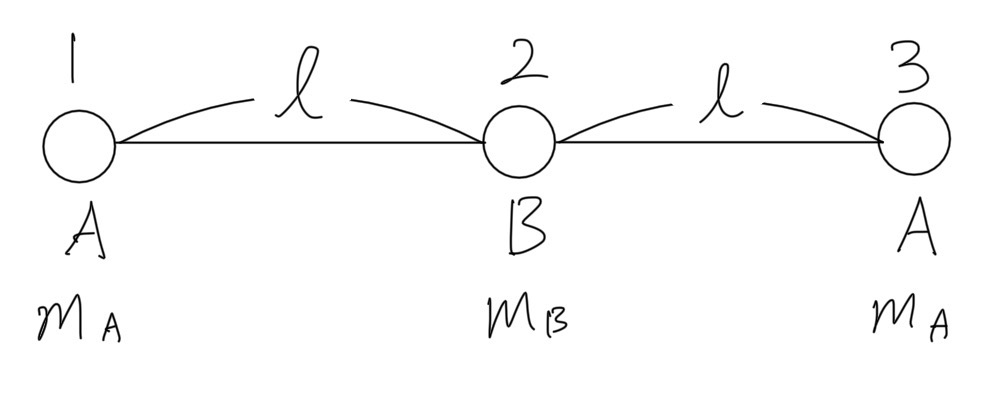
\includegraphics[width=0.6\textwidth]{5.png}
    \caption{直線状分子$A-B-A$の形}
    \label{fig:5}
  \end{figure}

  \section{Q2A-20（直線状分子$A-B-A$）}
  力学的平衡においては、2個の原子$A$と1個の原子$B$が直線状の$A-B-A$という形に並んだ3原子分子の微小振動を考察する。原子$A$と原子$B$の質量は、それぞれ、$m_A$と$m_B$とする。分子$A-B-A$が力学的平衡にあるとき、$A-B$の距離と$B-A$の距離はともに$l$であるとする。\hyperref[fig:5]{図5}を見てください。3 次元Descartes 座標系を、力学的平衡にある分子A−B−A の原子B が原点O に重なり、分子$A-B-A$のつくる線分がx軸に含まれるように用意する。
  力学的平衡において、点$(-l,0,0)$にある原子$A$を原子1と呼び、原点$O(0, 0, 0)$にある原子$B$を原子2と呼び、点$(l, 0, 0)$にある原子$A$を原子3と呼ぶことにする。$a = 1, 2, 3$に対して、原子$a$の平衡位置からのずれのベクトルを$\vect{u}_a = (u_{ax}, u_{ay}, u_{az})$とする。
  
  \subsection*{(i)}
  本小問では、直線状分子$A-B-A$の振動自由度を一般論から求める。この分子は3原子分子なので$n=3$である。また、直線状分子であるから、振動自由度は$3n-5=9-5=4$である。さらに、Q2A-19の結果より、直線に含まれる振動自由度は$n-1=2$であり、直線からはみ出る振動自由度は$2n-4=2$である。したがって、この直線状3原子分子には、直線に含まれる振動が2個、直線からはみ出る振動が2個ある。
  
  \subsection*{(ii)}
  本小問では、分子全体の並進運動と回転運動を含まない純粋な微小振動の制約条件を導く。原子1、2、3の平衡位置はそれぞれ$(-l,0,0)$、$(0,0,0)$、$(l,0,0)$である。ずれのベクトルを$\vect{u}_1,\vect{u}_2,\vect{u}_3$とする。並進を除く条件は、質量重み付きのずれの和が0であることなので、
  \begin{align*}
    m_A\vect{u}_1+m_B\vect{u}_2+m_A\vect{u}_3=\vect{0}。\tag{115}
  \end{align*}
  また、回転を除く条件は、平衡位置からの角運動量に対応する量が0であることなので、
  \begin{align*}
    m_A(-l,0,0)\times\vect{u}_1+m_B(0,0,0)\times\vect{u}_2+m_A(l,0,0)\times\vect{u}_3=\vect{0}。\tag{116}
  \end{align*}
  
  \subsection*{(iii)}
  本小問では、(115)式と(116)式は、見かけ上6個だが、実際には5個の独立な制約を与えることを説明する。\\
  (115)式はベクトル方程式なので3個の独立な制約を与える。一方、(116)式も形式的には3成分を持つが、平衡位置がすべて$x$軸上にあるため、外積の$x$成分は常に0である。したがって、(116)式から得られる独立な制約は$y,z$方向の回転に対応する2個だけである。よって、独立な制約の総数は$3+2=5$となり、一般論と一致する。
  
  \subsection*{(iv)}
  本小問では、制約条件を解いて、4個の一般座標$q_1,q_2,q_3,q_4$で原子のずれを表す。\\
  まず、独立変数として次の4つを選ぶ：
  \begin{align*}
    u_{1x}&=q_1,\tag{117}\\
    u_{3x}&=q_2,\tag{118}\\
    u_{1y}&=u_{3y}=q_3,\tag{119}\\
    u_{1z}&=u_{3z}=q_4。\tag{120}
  \end{align*}
  (115)式から、原子2のずれは次のようになる：
  \begin{align*}
    u_{2x}&=-\frac{m_A}{m_B}(q_1+q_2),\tag{121}\\
    u_{2y}&=-\frac{2m_A}{m_B}q_3,\tag{122}\\
    u_{2z}&=-\frac{2m_A}{m_B}q_4。\tag{123}
  \end{align*}
  したがって、ベクトルとして表すならば次のようになる：
  \begin{align*}
    \vect{u}_1&=(q_1,q_3,q_4),\tag{124}\\
    \vect{u}_2&=-\frac{m_A}{m_B}(q_1+q_2,2q_3,2q_4),\tag{125}\\
    \vect{u}_3&=(q_2,q_3,q_4)。\tag{126}
  \end{align*}
  また、一般座標ベクトルの列ベクトル$\vect{q}$も導入しておく：
  \begin{align*}
    \vect{q}=\begin{bmatrix}q_1\quad q_2\quad q_3\quad q_4\end{bmatrix}^t 。\tag{127}
  \end{align*}
  
  
  \subsection*{(v)}
  本小問では、この分子の微小振動の運動エネルギーを一般座標で表す。運動エネルギーは、
  \begin{align*}
    T=\frac{1}{2}m_A|\dot{\vect{u}}_1|^2+\frac{1}{2}m_B|\dot{\vect{u}}_2|^2+\frac{1}{2}m_A|\dot{\vect{u}}_3|^2
  \end{align*}
  である。(124)-(126)式を代入して整理する：
  \begin{align*}
    T=\frac{1}{2}\dot{\vect{q}}^{t}M\dot{\vect{q}}。\tag{128}
  \end{align*}
  ただし、
  \begin{align*}
    M=
    \begin{bmatrix}
      m_A+\frac{m_A^2}{m_B} & \frac{m_A^2}{m_B} & 0 & 0\\
      \frac{m_A^2}{m_B} & m_A+\frac{m_A^2}{m_B} & 0 & 0\\
      0 & 0 & 2m_A+\frac{4m_A^2}{m_B} & 0\\
      0 & 0 & 0 & 2m_A+\frac{4m_A^2}{m_B}
    \end{bmatrix}。\tag{129}
  \end{align*}
  平衡位置の周りに微小振動を行うこの分子のポテンシャルエネルギー$V$を、今までと同じに、平衡位置からのずれの2次の多項式として打ち切った調和近似で考察する。微小振動の振幅が小さくなるとき、調和近似はいくらでも正確になる。これから説明するように、ポテンシャルエネルギーVは2つの部分$V_1$と$V_2$からなる：
  \begin{align*}
    V=V_1+V_2。\tag{130}
  \end{align*}
  
  \subsection*{(vi)}
  本小問では、原子1と原子2、および原子2と原子3の間の結合距離が平衡値からずれることによるポテンシャル$V_1$を求める。このポテンシャルは、結合をバネとみなすFookの法則により模型化される：
  \begin{align*}
    V_1=\frac{1}{2}k_1|\vect{u}_1-\vect{u}_2|^2+\frac{1}{2}k_1|\vect{u}_2-\vect{u}_3|^2。
  \end{align*}
  まず、$\vect{u}_1-\vect{u}_2$を成分ごとに求める：
  \begin{align*}
    \vect{u}_1-\vect{u}_2=
    \left(\left(1+\frac{m_A}{m_B}\right)q_1+\frac{m_A}{m_B}q_2,\left(1+\frac{2m_A}{m_B}\right)q_3,\left(1+\frac{2m_A}{m_B}\right)q_4\right)。
  \end{align*}
  したがって、その大きさの2乗は、
  \begin{align*}
    |\vect{u}_1-\vect{u}_2|^2
    =
    \left\{\left(1+\frac{m_A}{m_B}\right)q_1+\frac{m_A}{m_B}q_2\right\}^2
    +\left(1+\frac{2m_A}{m_B}\right)^2q_3^2
    +\left(1+\frac{2m_A}{m_B}\right)^2q_4^2。
  \end{align*}
  同様に、$\vect{u}_2-\vect{u}_3$は、
  \begin{align*}
    \vect{u}_2-\vect{u}_3=
    -\left(\frac{m_A}{m_B}q_1+\left(1+\frac{m_A}{m_B}\right)q_2,\left(1+\frac{2m_A}{m_B}\right)q_3,\left(1+\frac{2m_A}{m_B}\right)q_4\right)。
  \end{align*}
  全体に負号が付いていても大きさの2乗には影響しないので、
  \begin{align*}
    |\vect{u}_2-\vect{u}_3|^2
    =
    \left\{\frac{m_A}{m_B}q_1+\left(1+\frac{m_A}{m_B}\right)q_2\right\}^2
    +\left(1+\frac{2m_A}{m_B}\right)^2q_3^2
    +\left(1+\frac{2m_A}{m_B}\right)^2q_4^2。
  \end{align*}
  よって、これらを$V_1$の定義に代入する：
  \begin{align*}
    V_1
    &=
    \frac{1}{2}k_1\left\{\left\{\left(1+\frac{m_A}{m_B}\right)q_1+\frac{m_A}{m_B}q_2\right\}^2
    +\left\{\frac{m_A}{m_B}q_1+\left(1+\frac{m_A}{m_B}\right)q_2\right\}^2\right\} \\
    &\quad
    +k_1\left(1+\frac{2m_A}{m_B}\right)^2q_3^2
    +k_1\left(1+\frac{2m_A}{m_B}\right)^2q_4^2。
  \end{align*}
  ここで、$q_1,q_2$を含む部分を展開する。$q_1^2$の係数は$\left(1+\frac{m_A}{m_B}\right)^2+\left(\frac{m_A}{m_B}\right)^2$であり、$q_2^2$の係数も同じである。また、$q_1q_2$の係数は$4\left(\frac{m_A}{m_B}+\frac{m_A^2}{m_B^2}\right)$である。したがって、
  \begin{align*}
    V_1
    &=
    \frac{1}{2}k_1\left(1+\frac{2m_A}{m_B}+\frac{2m_A^2}{m_B^2}\right)q_1^2
    +2k_1\left(\frac{m_A}{m_B}+\frac{m_A^2}{m_B^2}\right)q_1q_2
    +\frac{1}{2}k_1\left(1+\frac{2m_A}{m_B}+\frac{2m_A^2}{m_B^2}\right)q_2^2 \\
    &\quad
    +k_1\left(1+\frac{2m_A}{m_B}\right)^2q_3^2
    +k_1\left(1+\frac{2m_A}{m_B}\right)^2q_4^2。\tag{131}
  \end{align*}
  以上より、結合距離の変化を表すポテンシャル$V_1$が、一般座標$q_1,q_2,q_3,q_4$の2次形式として得られた。

  \subsection*{(vii)}
  本小問では、直線状分子$A-B-A$が折れ曲がったときに増加するポテンシャル$V_2$を導入する。原子1、2、3の実際の位置は、それぞれ$(-l,0,0)+\vect{u}_1$、$(0,0,0)+\vect{u}_2$、$(l,0,0)+\vect{u}_3$である。したがって、原子1から原子2へ向かうベクトルは次のように書ける：
  \begin{align*}
    (0,0,0)+\vect{u}_2-\{(-l,0,0)+\vect{u}_1\}。
  \end{align*}
  方向だけを取り出すために、このベクトルをその大きさで割ると、原子1から原子2へ向かう単位ベクトルは次のように表される：
  \begin{align*}
    \vect{n}_{12}=\frac{(0,0,0)+\vect{u}_2-\{(-l,0,0)+\vect{u}_1\}}{\left|(0,0,0)+\vect{u}_2-\{(-l,0,0)+\vect{u}_1\}\right|}。\tag{132}
  \end{align*}
  同様に、原子2から原子3へ向かう単位ベクトルは次のように表される：
  \begin{align*}
    \vect{n}_{23}=\frac{(l,0,0)+\vect{u}_3-\{(0,0,0)+\vect{u}_2\}}{\left|(l,0,0)+\vect{u}_3-\{(0,0,0)+\vect{u}_2\}\right|}。\tag{133}
  \end{align*}
  平衡状態では、3つの原子は$x$軸上に一直線に並んでいるので、$\vect{n}_{12}$と$\vect{n}_{23}$はいずれも$x$軸正方向を向く。したがって、分子が直線状であるという条件は、
  \begin{align*}
    \vect{n}_{12}=\vect{n}_{23}
  \end{align*}
  で表される。逆に、分子が折れ曲がると$\vect{n}_{12}$と$\vect{n}_{23}$の向きに差が生じるので、その折れ曲がりの大きさは$|\vect{n}_{12}-\vect{n}_{23}|$によって測ることができる。よって、直線状からのずれに対するポテンシャルを、調和近似として次のように模型化する：
  \begin{align*}
    V_2=\frac{1}{2}\tilde{k}_2l^2|\vect{n}_{12}-\vect{n}_{23}|^2。\tag{134}
  \end{align*}
  ここで、$\vect{n}_{12},\vect{n}_{23}$は単位ベクトルなので$|\vect{n}_{12}-\vect{n}_{23}|^2$は無次元である。そのため、$l^2$を掛けることで、$\tilde{k}_2$が通常のバネ定数と同じ次元を持つようにしている。以上より、分子の折れ曲がりを表すポテンシャル$V_2$は(134)式の形で与えられる。
  
  \subsection*{(viii)}
  本小問では、$\vect{n}_{12}$を平衡位置からのずれについて1次まで展開する。$\vect{e}_x=(1,0,0)$とし、
  \begin{align*}
    \vect{d}_{12}=\vect{u}_2-\vect{u}_1
  \end{align*}
  とおく。このとき、(132)式の分子は$l\vect{e}_x+\vect{d}_{12}$であるから、
  \begin{align*}
    \vect{n}_{12}=\frac{l\vect{e}_x+\vect{d}_{12}}{|l\vect{e}_x+\vect{d}_{12}|}
    =
    \frac{\vect{e}_x+\frac{1}{l}\vect{d}_{12}}{\sqrt{1+\frac{2}{l}\vect{e}_x\cdot\vect{d}_{12}+\frac{1}{l^2}|\vect{d}_{12}|^2}}
  \end{align*}
  と書ける。微小振動では$|\vect{d}_{12}|/l$が十分小さいので、分母の逆数を1次まで展開する：
  \begin{align*}
    \frac{1}{\sqrt{1+\frac{2}{l}\vect{e}_x\cdot\vect{d}_{12}+\frac{1}{l^2}|\vect{d}_{12}|^2}}
    =
    1-\frac{1}{l}\vect{e}_x\cdot\vect{d}_{12}+O\left(\frac{|u|^2}{l^2}\right)。
  \end{align*}
  これを$\vect{n}_{12}$に代入する：
  \begin{align*}
    \vect{n}_{12}
    &=
    \left(1-\frac{1}{l}\vect{e}_x\cdot\vect{d}_{12}\right)\left(\vect{e}_x+\frac{1}{l}\vect{d}_{12}\right)+O\left(\frac{|u|^2}{l^2}\right) \\
    &=
    \vect{e}_x+\frac{1}{l}\vect{d}_{12}-\frac{1}{l}(\vect{e}_x\cdot\vect{d}_{12})\vect{e}_x+O\left(\frac{|u|^2}{l^2}\right) \\
    &=
    \vect{e}_x+\frac{1}{l}(\vect{e}_y\otimes\vect{e}_y+\vect{e}_z\otimes\vect{e}_z)(\vect{u}_2-\vect{u}_1)+O\left(\frac{|u|^2}{l^2}\right)。\tag{135}
  \end{align*}
  
  \subsection*{(ix)}
  本小問では、$\vect{n}_{23}$を同様に1次まで展開する。ここで、
  \begin{align*}
    \vect{d}_{23}=\vect{u}_3-\vect{u}_2
  \end{align*}
  とおくと、原子2から原子3へ向かうベクトルは$l\vect{e}_x+\vect{d}_{23}$である。したがって、前小問と同じ展開により、
  \begin{align*}
    \vect{n}_{23}
    =
    \vect{e}_x+\frac{1}{l}(\vect{e}_y\otimes\vect{e}_y+\vect{e}_z\otimes\vect{e}_z)(\vect{u}_3-\vect{u}_2)+O\left(\frac{|u|^2}{l^2}\right)
  \end{align*}
  を得る。よって、
  \begin{align*}
    \vect{n}_{23}=\vect{e}_x+\frac{1}{l}(\vect{e}_y\otimes\vect{e}_y+\vect{e}_z\otimes\vect{e}_z)(\vect{u}_3-\vect{u}_2)+O\left(\frac{|u|^2}{l^2}\right)。\tag{136}
  \end{align*}
  
  \subsection*{(x)}
  本小問では、$\vect{n}_{12}-\vect{n}_{23}$を求める。(135)式と(136)式を用いる：
  \begin{align*}
    \vect{n}_{12}-\vect{n}_{23}
    &=
    \frac{1}{l}(\vect{e}_y\otimes\vect{e}_y+\vect{e}_z\otimes\vect{e}_z)\{(\vect{u}_2-\vect{u}_1)-(\vect{u}_3-\vect{u}_2)\}+O\left(\frac{|u|^2}{l^2}\right) \\
    &=
    -\frac{1}{l}(\vect{e}_y\otimes\vect{e}_y+\vect{e}_z\otimes\vect{e}_z)(\vect{u}_1-2\vect{u}_2+\vect{u}_3)+O\left(\frac{|u|^2}{l^2}\right)。
  \end{align*}
  ここで、$\vect{e}_y\otimes\vect{e}_y+\vect{e}_z\otimes\vect{e}_z$は$y,z$成分だけを取り出す写像である。したがって、成分で書けば次のようになる：
  \begin{align*}
    \vect{n}_{12}-\vect{n}_{23}
    =
    -\frac{1}{l}(0,u_{1y}-2u_{2y}+u_{3y},u_{1z}-2u_{2z}+u_{3z})+O\left(\frac{|u|^2}{l^2}\right)。\tag{137}
  \end{align*}
  
  \subsection*{(xi)}
  本小問では、調和近似のもとで$V_2$を一般座標$q_3,q_4$で表す。(137)式を(134)式に代入し、2次までを残す：
  \begin{align*}
    V_2=\frac{1}{2}\tilde{k}_2\{(u_{1y}-2u_{2y}+u_{3y})^2+(u_{1z}-2u_{2z}+u_{3z})^2\}。
  \end{align*}
  ここで、制約条件から得たずれのベクトルの表示を用いる：
  \begin{align*}
    \vect{u}_1=(q_1,q_3,q_4),\qquad
    \vect{u}_2=-\frac{m_A}{m_B}(q_1+q_2,2q_3,2q_4),\qquad
    \vect{u}_3=(q_2,q_3,q_4)。
  \end{align*}
  まず、$y$成分について計算する：
  \begin{align*}
    u_{1y}-2u_{2y}+u_{3y}
    =
    q_3-2\left(-\frac{2m_A}{m_B}q_3\right)+q_3
    =
    2\left(1+\frac{2m_A}{m_B}\right)q_3。
  \end{align*}
  同様に、$z$成分についても計算する：
  \begin{align*}
    u_{1z}-2u_{2z}+u_{3z}
    =
    q_4-2\left(-\frac{2m_A}{m_B}q_4\right)+q_4
    =
    2\left(1+\frac{2m_A}{m_B}\right)q_4。
  \end{align*}
  これらを$V_2$に代入する：
  \begin{align*}
    V_2
    &=
    \frac{1}{2}\tilde{k}_2\left\{4\left(1+\frac{2m_A}{m_B}\right)^2q_3^2+4\left(1+\frac{2m_A}{m_B}\right)^2q_4^2\right\} \\
    &=
    2\tilde{k}_2\left(1+\frac{2m_A}{m_B}\right)^2q_3^2
    +2\tilde{k}_2\left(1+\frac{2m_A}{m_B}\right)^2q_4^2。\tag{138}
  \end{align*}
  
  \subsection*{(xii)}
  本小問では、$V_1$と$V_2$を合わせた全ポテンシャル$V$を2次形式として表す。全ポテンシャルは、距離変化に対応する$V_1$と、曲がりに対応する$V_2$の和である：
  \begin{align*}
    V=V_1+V_2。
  \end{align*}
  まず、(vi)で得た$V_1$は次である：
  \begin{align*}
    V_1
    &=
    \frac{1}{2}k_1\left(1+\frac{2m_A}{m_B}+\frac{2m_A^2}{m_B^2}\right)q_1^2
    +2k_1\left(\frac{m_A}{m_B}+\frac{m_A^2}{m_B^2}\right)q_1q_2
    +\frac{1}{2}k_1\left(1+\frac{2m_A}{m_B}+\frac{2m_A^2}{m_B^2}\right)q_2^2 \\
    &\quad
    +k_1\left(1+\frac{2m_A}{m_B}\right)^2q_3^2
    +k_1\left(1+\frac{2m_A}{m_B}\right)^2q_4^2。
  \end{align*}
  これに(138)式の$V_2$を加える。$q_1,q_2$に関する項は$V_1$からのみ来る。一方、$q_3^2,q_4^2$の係数は次のようにまとまる：
  \begin{align*}
    k_1\left(1+\frac{2m_A}{m_B}\right)^2+2\tilde{k}_2\left(1+\frac{2m_A}{m_B}\right)^2
    =
    2\left(\frac{1}{2}k_1+\tilde{k}_2\right)\left(1+\frac{2m_A}{m_B}\right)^2。
  \end{align*}
  ここで、
  \begin{align*}
    k_2=\frac{1}{2}k_1+\tilde{k}_2\tag{141}
  \end{align*}
  と定めると、$q_3^2,q_4^2$の係数は$2k_2(1+2m_A/m_B)^2$である。したがって、全ポテンシャルは次のようになる：
  \begin{align*}
    V
    &=
    \frac{1}{2}k_1\left(1+\frac{2m_A}{m_B}+\frac{2m_A^2}{m_B^2}\right)q_1^2
    +2k_1\left(\frac{m_A}{m_B}+\frac{m_A^2}{m_B^2}\right)q_1q_2
    +\frac{1}{2}k_1\left(1+\frac{2m_A}{m_B}+\frac{2m_A^2}{m_B^2}\right)q_2^2 \\
    &\quad
    +2k_2\left(1+\frac{2m_A}{m_B}\right)^2q_3^2
    +2k_2\left(1+\frac{2m_A}{m_B}\right)^2q_4^2。
  \end{align*}
  これを
  \begin{align*}
    V=\frac{1}{2}\vect{q}^{\mathrm{t}}N\vect{q}\tag{139}
  \end{align*}
  の形に書く。係数を比較すると、行列$N$は次のように定まる：
  \begin{align*}
    N=
    \begin{pmatrix}
      k_1\left(1+\frac{2m_A}{m_B}+\frac{2m_A^2}{m_B^2}\right) & 2k_1\left(\frac{m_A}{m_B}+\frac{m_A^2}{m_B^2}\right) & 0 & 0 \\
      2k_1\left(\frac{m_A}{m_B}+\frac{m_A^2}{m_B^2}\right) & k_1\left(1+\frac{2m_A}{m_B}+\frac{2m_A^2}{m_B^2}\right) & 0 & 0 \\
      0 & 0 & 4k_2\left(1+\frac{2m_A}{m_B}\right)^2 & 0 \\
      0 & 0 & 0 & 4k_2\left(1+\frac{2m_A}{m_B}\right)^2
    \end{pmatrix}。\tag{140}
  \end{align*}
  
  \subsection*{(xiii)}
  本小問では、4個の基準振動の角振動数を決める方程式を確認する。微小振動のLagrange関数は、
  \begin{align*}
    L=\frac{1}{2}\dot{\vect{q}}^{\mathrm{t}}M\dot{\vect{q}}-\frac{1}{2}\vect{q}^{\mathrm{t}}N\vect{q}
  \end{align*}
  の形で書ける。したがって、Euler-Lagrange方程式は、
  \begin{align*}
    M\ddot{\vect{q}}+N\vect{q}=\vect{0}
  \end{align*}
  である。基準振動として$\vect{q}(t)=\vect{q}_i\cos(\omega_i t+\theta_i)$を代入する：
  \begin{align*}
    (N-\omega_i^2M)\vect{q}_i=\vect{0}。
  \end{align*}
  非自明な解$\vect{q}_i\neq\vect{0}$が存在するためには、係数行列の行列式が0でなければならない。よって：
  \begin{align*}
    \det(N-\omega_i^2M)=0\qquad(i=1,2,3,4)。\tag{142}
  \end{align*}
  
  \subsection*{(xiv)}
  本小問では、直線からはみ出る2つの基準振動の角振動数を求める。$q_3,q_4$に関する部分では、$M$と$N$はともに対角であり、さらに$q_3$と$q_4$に対する係数が等しい。したがって、$q_3$方向と$q_4$方向の振動は同じ角振動数を持つ。$q_3$成分について、対応する$M,N$の成分を読む：
  \begin{align*}
    M_{33}=2m_A+\frac{4m_A^2}{m_B}=2m_A\left(1+\frac{2m_A}{m_B}\right),
    \qquad
    N_{33}=4k_2\left(1+\frac{2m_A}{m_B}\right)^2。
  \end{align*}
  したがって、$q_3$方向の角振動数は次のように求まる：
  \begin{align*}
    \omega_3^2=\frac{N_{33}}{M_{33}}=\frac{4k_2\left(1+\frac{2m_A}{m_B}\right)^2}{2m_A\left(1+\frac{2m_A}{m_B}\right)}=\frac{2k_2(2m_A+m_B)}{m_Am_B}。
  \end{align*}
  同じ計算が$q_4$方向にも成り立つので、
  \begin{align*}
    \omega_3=\omega_4=\sqrt{\frac{2k_2(2m_A+m_B)}{m_Am_B}}。\tag{143}
  \end{align*}
  以上より、直線からはみ出る2つの基準振動は縮退していることが示された。
  
  \subsection*{(xv)}
  本小問では、直線に含まれる残り2個の基準振動の角振動数を決める方程式を取り出す。$q_1,q_2$の部分だけを取り出すと、$M,N$の該当する$2\times2$成分は次のようになる：
  \begin{align*}
    M_\parallel=
    \begin{pmatrix}
      m_A+\frac{m_A^2}{m_B} & \frac{m_A^2}{m_B} \\
      \frac{m_A^2}{m_B} & m_A+\frac{m_A^2}{m_B}
    \end{pmatrix},
  \qquad
    N_\parallel=
    k_1
    \begin{pmatrix}
      1+\frac{2m_A}{m_B}+\frac{2m_A^2}{m_B^2} & 2\left(\frac{m_A}{m_B}+\frac{m_A^2}{m_B^2}\right) \\
      2\left(\frac{m_A}{m_B}+\frac{m_A^2}{m_B^2}\right) & 1+\frac{2m_A}{m_B}+\frac{2m_A^2}{m_B^2}
    \end{pmatrix}。
  \end{align*}
  したがって、$\omega_1,\omega_2$は次の行列式方程式によって定まる：
  \begin{align*}
    \det(N_\parallel-\omega_i^2M_\parallel)=0\qquad(i=1,2)。\tag{144}
  \end{align*}
  
  \subsection*{(xvi)}
  本小問では、(144)式を解いて$\omega_1,\omega_2$を求める。$M_\parallel,N_\parallel$はいずれも
  \begin{align*}
    \begin{pmatrix}
      A & B \\
      B & A
    \end{pmatrix}
  \end{align*}
  の形をしているので、対称なベクトル$(1,1)$と反対称なベクトル$(1,-1)$で同時に対角化できる。まず、対称モード$(1,1)$を考える。このとき、$M_\parallel$の固有値は次のようになる：
  \begin{align*}
    \left(m_A+\frac{m_A^2}{m_B}\right)+\frac{m_A^2}{m_B}=m_A+\frac{2m_A^2}{m_B}=m_A\left(1+\frac{2m_A}{m_B}\right)。
  \end{align*}
  また、$N_\parallel$の固有値は次のようになる：
  \begin{align*}
    k_1\left(1+\frac{2m_A}{m_B}+\frac{2m_A^2}{m_B^2}+2\frac{m_A}{m_B}+2\frac{m_A^2}{m_B^2}\right)
    =
    k_1\left(1+\frac{2m_A}{m_B}\right)^2。
  \end{align*}
  したがって、対称モードの角振動数は次のようになる：
  \begin{align*}
    \omega_1^2=\frac{k_1\left(1+\frac{2m_A}{m_B}\right)^2}{m_A\left(1+\frac{2m_A}{m_B}\right)}=\frac{k_1(2m_A+m_B)}{m_Am_B}。
  \end{align*}
  次に、反対称モード$(1,-1)$を考える。このとき、$M_\parallel$の固有値は次のようになる：
  \begin{align*}
    \left(m_A+\frac{m_A^2}{m_B}\right)-\frac{m_A^2}{m_B}=m_A。
  \end{align*}
  また、$N_\parallel$の固有値は次のようになる：
  \begin{align*}
    k_1\left(1+\frac{2m_A}{m_B}+\frac{2m_A^2}{m_B^2}-2\frac{m_A}{m_B}-2\frac{m_A^2}{m_B^2}\right)=k_1。
  \end{align*}
  したがって、反対称モードの角振動数は次のようになる：
  \begin{align*}
    \omega_2^2=\frac{k_1}{m_A}。
  \end{align*}
  以上より、
  \begin{align*}
    \omega_1&=\sqrt{\frac{k_1(2m_A+m_B)}{m_Am_B}},\tag{145}\\
    \omega_2&=\sqrt{\frac{k_1}{m_A}}。\tag{146}
  \end{align*}
  
  \subsection*{(xvii)}
  本小問では、一般座標$\vect{q}=(q_1,q_2,q_3,q_4)$で見た4つの基準振動の振幅ベクトルを求める。前小問より、$q_1,q_2$に関する基準振動は対称モードと反対称モードであり、$q_3,q_4$は互いに混ざらず独立に振動する。したがって、振幅ベクトルは次のように取れる：
  \begin{align*}
    \vect{q}_1&\propto(1,1,0,0)^t,\tag{147}\\
    \vect{q}_2&\propto(1,-1,0,0)^t,\tag{148}\\
    \vect{q}_3&\propto(0,0,1,0)^t,\tag{149}\\
    \vect{q}_4&\propto(0,0,0,1)^t。\tag{150}
  \end{align*}
  
  \subsection*{(xviii)}
  本小問では、基準振動モード1を、もとの原子のずれのベクトルで表す。モード1では$\vect{q}_1\propto(1,1,0,0)^t$であるから、$q_1=q_2$、$q_3=q_4=0$とおけばよい。この条件を
  \begin{align*}
    \vect{u}_1=(q_1,q_3,q_4),\qquad
    \vect{u}_2=-\frac{m_A}{m_B}(q_1+q_2,2q_3,2q_4),\qquad
    \vect{u}_3=(q_2,q_3,q_4)
  \end{align*}
  に代入する：
  \begin{align*}
    \vect{u}_1\propto(1,0,0),\qquad
    \vect{u}_2\propto\left(-\frac{2m_A}{m_B},0,0\right),\qquad
    \vect{u}_3\propto(1,0,0)。\tag{151}
  \end{align*}
  このモードでは、両端の原子$A$が同じ向きに動き、中央の原子$B$がそれと反対向きに動く。
  
  \subsection*{(xix)}
  本小問では、基準振動モード2を、もとの原子のずれのベクトルで表す。モード2では$\vect{q}_2\propto(1,-1,0,0)$であるから、$q_1=-q_2$、$q_3=q_4=0$とおけばよい。このとき$q_1+q_2=0$であるから、原子2の変位は消える。したがって：
  \begin{align*}
    \vect{u}_1\propto(1,0,0),\qquad
    \vect{u}_2\propto(0,0,0),\qquad
    \vect{u}_3\propto(-1,0,0)。\tag{152}
  \end{align*}
  このモードでは、中央の原子$B$は静止し、両端の原子$A$だけが互いに反対向きに動く。
  
  \subsection*{(xx)}
  本小問では、基準振動モード3を、もとの原子のずれのベクトルで表す。モード3では$q_3$だけが非零であり、$q_1=q_2=q_4=0$である。これを原子のずれの表示に代入する：
  \begin{align*}
    \vect{u}_1\propto(0,1,0),\qquad
    \vect{u}_2\propto\left(0,-\frac{2m_A}{m_B},0\right),\qquad
    \vect{u}_3\propto(0,1,0)。\tag{153}
  \end{align*}
  このモードは、分子軸から$y$方向にはみ出る振動である。
  
  \subsection*{(xxi)}
  本小問では、基準振動モード4を、もとの原子のずれのベクトルで表す。モード4では$q_4$だけが非零であり、$q_1=q_2=q_3=0$である。これを原子のずれの表示に代入する：
  \begin{align*}
    \vect{u}_1\propto(0,0,1),\qquad
    \vect{u}_2\propto\left(0,0,-\frac{2m_A}{m_B}\right),\qquad
    \vect{u}_3\propto(0,0,1)。\tag{154}
  \end{align*}
  このモードは、分子軸から$z$方向にはみ出る振動である。
  
  \subsection*{(xxii)}
  本小問では、基準振動モード1から4を、直線に含まれる振動と直線からはみ出る振動に分類する。モード1とモード2では、原子のずれのベクトルは$x$成分だけを持つ。したがって、これらは分子軸である$x$軸に沿った振動であり、直線に含まれる振動である。モード1では両端の原子$A$が同じ向きに動き、中央の原子$B$が反対向きに動くので、分子の中心に関して反対称な振動である。モード2では両端の原子$A$が互いに反対向きに動き、中央の原子$B$は静止するので、分子の中心に関して対称な振動である。
  
  一方、モード3とモード4では、原子のずれのベクトルはそれぞれ$y$成分、$z$成分を持つ。したがって、これらは分子軸からはみ出る振動である。以上より、分類は次のように書ける：
  \begin{align*}
    \begin{array}{ll}
      \text{基準振動モード1} & ：\text{直線に含まれる振動。分子の中心に関して反対称な振動。}\\
      \text{基準振動モード2} & ：\text{直線に含まれる振動。分子の中心に関して対称な振動。}\\
      \text{基準振動モード3} & ：\text{直線からはみ出る振動。}\\
      \text{基準振動モード4} & ：\text{直線からはみ出る振動。}
    \end{array}\tag{155}
  \end{align*}
  また、モード3とモード4は、平衡状態の分子軸である$x$軸に垂直な$yz$平面内の回転対称性により縮退している。すなわち、$y$方向にはみ出る振動と$z$方向にはみ出る振動は、座標軸の取り方を$yz$平面内で回転することにより互いに移り合うため、同じ角振動数を持つ。
  \subsection*{(xxiii)}
  本小問では、(xviii)から(xxi)で得た4つの基準振動モードを、原子のずれの向きとして図示する。各モードでのずれの比例関係は、次のようにまとめられる：
  \begin{align*}
    \begin{array}{ll}
      \text{モード1} & ：\vect{u}_1\propto(1,0,0),\quad \vect{u}_2\propto\left(-\frac{2m_A}{m_B},0,0\right),\quad \vect{u}_3\propto(1,0,0),\\
      \text{モード2} & ：\vect{u}_1\propto(1,0,0),\quad \vect{u}_2\propto(0,0,0),\quad \vect{u}_3\propto(-1,0,0),\\
      \text{モード3} & ：\vect{u}_1\propto(0,1,0),\quad \vect{u}_2\propto\left(0,-\frac{2m_A}{m_B},0\right),\quad \vect{u}_3\propto(0,1,0),\\
      \text{モード4} & ：\vect{u}_1\propto(0,0,1),\quad \vect{u}_2\propto\left(0,0,-\frac{2m_A}{m_B}\right),\quad \vect{u}_3\propto(0,0,1)。
    \end{array}
  \end{align*}
  ここで、モード1とモード2は分子軸である$x$軸方向の振動であり、モード3とモード4は分子軸からはみ出る振動である。これらを矢印で表すと、次のようになる：
  
  \begin{figure}[H]
    \centering
    \begin{tikzpicture}[scale=1.0]
      % 共通設定
      \tikzset{
        atomA/.style={circle, draw, minimum size=8mm},
        atomB/.style={circle, draw, minimum size=8mm},
        arr/.style={->, thick},
        smallarr/.style={->, thick},
      }
  
      % mode 1
      \node at (-3.5,3.6) {モード1};
      \node[atomA] (A1) at (-1.8,3.6) {$A$};
      \node[atomB] (B1) at (0,3.6) {$B$};
      \node[atomA] (C1) at (1.8,3.6) {$A$};
      \draw (-1.4,3.6) -- (-0.4,3.6);
      \draw (0.4,3.6) -- (1.4,3.6);
      \draw[arr] (-1.8,3.05) -- (-1.25,3.05);
      \draw[arr] (1.8,3.05) -- (2.35,3.05);
      \draw[arr] (0,4.25) -- (-0.85,4.25);
      \node[right] at (2.55,3.05) {$x$方向};
      \node at (0,2.75) {両端の$A$が同方向、中央の$B$が逆方向に動く。};
  
      % mode 2
      \node at (-3.5,1.2) {モード2};
      \node[atomA] (A2) at (-1.8,1.2) {$A$};
      \node[atomB] (B2) at (0,1.2) {$B$};
      \node[atomA] (C2) at (1.8,1.2) {$A$};
      \draw (-1.4,1.2) -- (-0.4,1.2);
      \draw (0.4,1.2) -- (1.4,1.2);
      \draw[arr] (-1.8,0.65) -- (-1.25,0.65);
      \draw[arr] (1.8,0.65) -- (1.25,0.65);
      \node at (0,1.85) {静止};
      \node at (0,0.35) {両端の$A$が逆方向に動き、中央の$B$は静止する。};
  
      % mode 3
      \node at (-3.5,-1.2) {モード3};
      \node[atomA] (A3) at (-1.8,-1.2) {$A$};
      \node[atomB] (B3) at (0,-1.2) {$B$};
      \node[atomA] (C3) at (1.8,-1.2) {$A$};
      \draw (-1.4,-1.2) -- (-0.4,-1.2);
      \draw (0.4,-1.2) -- (1.4,-1.2);
      \draw[arr] (-1.8,-1.75) -- (-1.8,-1.1);
      \draw[arr] (1.8,-1.75) -- (1.8,-1.1);
      \draw[arr] (0,-0.55) -- (0,-1.4);
      \node[right] at (2.25,-1.4) {$y$方向};
      \node at (0,-2.05) {両端の$A$が$y$方向、中央の$B$が逆方向に動く。};
  
      % mode 4
      \node at (-3.5,-3.6) {モード4};
      \node[atomA] (A4) at (-1.8,-3.6) {$A$};
      \node[atomB] (B4) at (0,-3.6) {$B$};
      \node[atomA] (C4) at (1.8,-3.6) {$A$};
      \draw (-1.4,-3.6) -- (-0.4,-3.6);
      \draw (0.4,-3.6) -- (1.4,-3.6);
      \node at (-1.8,-4.25) {$\odot$};
      \node at (1.8,-4.25) {$\odot$};
      \node at (0,-2.95) {$\otimes$};
      \node[right] at (2.25,-4.05) {$z$方向};
      \node at (0,-4.55) {両端の$A$が紙面手前、中央の$B$が紙面奥向きに動く。};
    \end{tikzpicture}
    \caption*{直線状分子$A-B-A$の基準振動モード}
    \label{fig:q2a20-normal-modes}
  \end{figure}

  \clearpage
  \part{自己採点表}
  \begin{table}[H]
    \centering
    \caption{自己採点表}
    \begin{tabular}{c|c|c}
      \hline
      問題番号 & 小問 & 自己評価 \\
      \hline
      Q2A-1 & 全小問 & ○ \\
      Q2A-2 & 全小問 & ○ \\
      Q2A-3 & (i)〜(ix), (xi) & ○ \\
      Q2A-3 & (x), (xii) & × \\
      Q2A-4 & 全小問 & ○ \\
      Q2A-5 & 全小問 & ○ \\
      Q2A-6 & 全小問 & ○ \\
      Q2A-7 & 全小問 & ○ \\
      Q2A-10 & (i) & ○ \\
      Q2A-10 & (ii) & × \\
      Q2A-11 & 全小問 & ○ \\
      Q2A-12 & 全小問 & ○ \\
      Q2A-13 & 全小問 & ○ \\
      Q2A-14 & 全小問 & ○ \\
      Q2A-15 & 全小問 & ○ \\
      Q2A-16 & 全小問 & ○ \\
      Q2A-17 & 全小問 & ○ \\
      Q2A-18 & 全小問 & ○ \\
      Q2A-19 & 全小問 & ○ \\
      Q2A-20 & 全小問 & ○ \\
      \hline
    \end{tabular}
  \end{table}


\end{document}